\documentclass{article}

% NeurIPS 2026 — Evaluations & Datasets track, supplementary material
\usepackage[eandd]{neurips_2026}

\usepackage[utf8]{inputenc}
\usepackage[T1]{fontenc}
\usepackage{hyperref}
\usepackage{url}
\usepackage{booktabs}
\usepackage{amsfonts}
\usepackage{amsmath}
\usepackage{amssymb}
\usepackage{nicefrac}
\usepackage{microtype}
\usepackage{xcolor}
\usepackage{calc}
\usepackage{graphicx}
\graphicspath{{figures/}{../figures/}}
\usepackage{longtable}
\usepackage{array}
\usepackage{caption}
\usepackage{ragged2e}
\usepackage{tikz}
\usetikzlibrary{positioning, decorations.pathreplacing, calc, fit}

% Pandoc compatibility
\providecommand{\tightlist}{\setlength{\itemsep}{0pt}\setlength{\parskip}{0pt}}
\providecommand{\real}[1]{#1}

\title{Supplementary Material:\\
When Does Workflow Conditioning Help Remaining Surgery Duration
Prediction? A Variability-Scaling Study on MultiBypass140 and Cholec80}

% Anonymous for double-blind review
\author{%
  Anonymous Author(s) \\
  Affiliation(s) \\
  Address(es) \\
  \texttt{anonymous@anonymous.edu}
}

\begin{document}

\maketitle

\begin{abstract}
\noindent
This document is the supplementary material accompanying the main paper.
It contains content cut from the 9-page main body for length, organized
as Appendices A--H plus Appendix Z. The references list is also
reproduced here for self-contained reading. No headline empirical claim
from the main paper depends on material in this supplement; the
appendices provide reproducibility details, ablations,
statistical-significance tests, per-fold tables, extended discussion,
and additional explanatory figures.
\end{abstract}

\tableofcontents
\newpage

% All Appendices A through F + Z (auto-generated from review_manuscript.md
% by paper/scripts/build_latex.py)
\section{Appendix A --- Implementation
Details}\label{appendix-a-implementation-details}

\textbf{Repository.} \texttt{brsd\_lib} (clean-room Python library) and
\texttt{lambda\_setup} (training and preprocessing scripts) implement
the full pipeline. Cluster artifacts
(\texttt{*\_kmeans\_artifacts.json}) persist the TF-IDF vocabulary, IDF
weights, PCA components and mean, k-means centroids, and a
phase-id-to-name mapping in a single JSON file --- sufficient to
reproduce the offline cluster assignment from any phase sequence
(including a sequence predicted by the trained model's phase head at
inference).

\textbf{Sanity check.} We verify that our online cluster pipeline
reproduces the offline cluster assignment exactly when fed the
ground-truth phase sequence: on all 140 MultiBypass140 fold-0 videos the
online argmax-posterior cluster matches the offline k-means assignment
(140/140 = 100\%). Any error in the causal-at-inference variant
therefore reflects phase-head prediction error, not clustering math.

\textbf{Prefix-cluster fallback statistics.} Per-clip, the
prefix-cluster pipeline either returns (i) a non-trivial soft posterior
($\geq$ 2 unique phases in prefix), (ii) a fallback to the video's oracle
cluster (\textless{} 2 unique phases), or (iii) a uniform posterior (no
in-vocabulary bigrams; never observed in practice). On MultiBypass140
fold 0: 153,111 clips, 59.15\% match oracle (excluding fallback), 7.25\%
fallback. On Cholec80: 29,096 clips, 50.31\% match, 7.60\% fallback. The
50--60\% per-clip match rate shows that the prefix-derived cluster is
\emph{not} a noisy copy of the oracle --- 40--50\% of clips receive a
different cluster identifier under the causal pipeline, and the model
learns across both regimes during training.

\textbf{Hardware utilization.} All experiments were run on Lambda Cloud
GH200 instances (us-east-3 region) with a shared persistent NFS
filesystem. Across the full project --- including the strict-protocol
training (Run 033, 034, 037), the 5-fold extension (Run 038/039/040, 36
runs), the strict pixel-only causal evaluation (Run 035), the
oracle-baseline matched-metric evaluation (Run 044), the temperature
sweep (Run 041), the shuffled-token re-evaluation (Run 045), the strict
Cholec80 mini-run (Run 046), and the centered-window legacy runs (Run
010, 022, 023, 026, 027, 028) --- total GPU-time was approximately 370
GH200-hours over a \textasciitilde7-day window across 4 parallel
instances, at an aggregate cloud cost of approximately \$850 USD (at
\$2.29/hr). The reproducibility package (Appendix Z) re-runs any single
configuration in 1--2 GH200-hours.

\section{Appendix B --- Hyperparameter sensitivity and the smoother}\label{appendix-b-hyperparameter-sensitivity-and-the-smoother}

\textbf{Cluster count \(K\).} We treat \(K\) as a hyperparameter chosen
by inspecting cluster-size balance before any RSD evaluation. On MB140
we considered \(K \in \{4, 6, 8\}\) and selected \(K = 6\) (balanced
38/27/25/23/17/10); \(K = 4\) collapses one cluster to 50+ videos and
\(K = 8\) produces singletons. \textbf{PCA dimensionality.} TF-IDF
dimensionality is 63 on MB140 and 10 on Cholec80; we project to 16 PCA
components, with cluster assignments robust to \(\pm 8\) components.
\textbf{Cluster-posterior temperature.} The causal pipeline uses
softmax-of-negative-squared-distance with \(\tau =
0.01\) (effectively hard argmax with small uncertainty margin). A
5-point sweep on Run 033 strict decoupled-oracle seed 42 (Run 041:
\(\tau \in \{0.01, 0.05, 0.1, 0.5, 1.0\}\), evaluated under the
matched-metric pixel-only causal pipeline of the main-text pixel-only causal evaluation) produced val MAE in
the range 11.74--11.88 min --- total spread \textbf{0.15 min}, within
typical cross-seed noise. Temperature is therefore not a useful knob for
closing the oracle-to-causal gap; production \(\tau = 0.01\) is
essentially optimal. \textbf{Phase head.} Macro per-frame accuracy 0.78
on MB140 fold 0 val (Run 010 seed 42), per-class range 0.61--0.93.

\textbf{Adam-style smoother (\texttt{brsd\_lib.smoothing}).} Maintains
exponentially weighted first and second moments of the prediction
sequence and blends each new prediction with the moving average in
proportion to local variance: \[
m_t = \beta_1 m_{t-1} + (1{-}\beta_1) \hat y_t,\;\;
v_t = \beta_2 v_{t-1} + (1{-}\beta_2)(\hat y_t - \hat m_t)^2,
\] \[
\alpha_t = \frac{\tau^2}{\tau^2 + \hat v_t + \varepsilon},\;\;
\tilde y_t = \alpha_t \hat y_t + (1{-}\alpha_t)\hat m_t,\;\;
y^*_t = \min(\tilde y_t, y^*_{t-1}),
\] where \(\hat m_t, \hat v_t\) are bias-corrected \citep{kingma2015adam}.
This generalizes per-video isotonic regression by adapting smoothing
strength to local prediction variance.

\section{Appendix C --- Per-Fold and Per-Seed Tables}\label{appendix-c-per-fold-and-per-seed-tables}

\subsection{C.1 MultiBypass140 strict-protocol 5-fold $\times$ 3-seed
extension (Phase
E)}\label{c.1-multibypass140-strict-protocol-5-fold-3-seed-extension-phase-e}

\paragraph{C.1.1 Fold-0 headline (Run
033)}\label{c.1.1-fold-0-headline-run-033}

Per-seed validation MAE under the main-text within-center metric (clip-weighted, fixed
training-set-mean denorm, \textasciitilde110 min):

\begin{longtable}[]{@{}
  >{\raggedright\arraybackslash}p{(\linewidth - 8\tabcolsep) * \real{0.1579}}
  >{\raggedleft\arraybackslash}p{(\linewidth - 8\tabcolsep) * \real{0.2105}}
  >{\raggedleft\arraybackslash}p{(\linewidth - 8\tabcolsep) * \real{0.2105}}
  >{\raggedleft\arraybackslash}p{(\linewidth - 8\tabcolsep) * \real{0.2105}}
  >{\raggedleft\arraybackslash}p{(\linewidth - 8\tabcolsep) * \real{0.2105}}@{}}
\toprule\noalign{}
\begin{minipage}[b]{\linewidth}\raggedright
Configuration
\end{minipage} & \begin{minipage}[b]{\linewidth}\raggedleft
Seed 42
\end{minipage} & \begin{minipage}[b]{\linewidth}\raggedleft
Seed 123
\end{minipage} & \begin{minipage}[b]{\linewidth}\raggedleft
Seed 777
\end{minipage} & \begin{minipage}[b]{\linewidth}\raggedleft
Mean $\pm$ std
\end{minipage} \\
\midrule\noalign{}
\endhead
\bottomrule\noalign{}
\endlastfoot
Strict no-token & 13.17 & 13.10 & 12.83 & \textbf{13.03 $\pm$ 0.18} \\
Strict oracle & 12.18 & 12.23 & 12.36 & \textbf{12.26 $\pm$ 0.09} \\
\textbf{Strict decoupled-oracle} & \textbf{12.32} & \textbf{12.19} &
\textbf{12.04} & \textbf{12.18 $\pm$ 0.14} \\
\end{longtable}

\paragraph{C.1.2 Per-fold mean $\pm$ std across all 5
folds}\label{c.1.2-per-fold-mean-std-across-all-5-folds}

Phase E ran the same three conditions on folds 1--4 $\times$ 3 seeds (36
training runs); fold 0 reference is Run 033. Validation MAE in minutes:

\begin{longtable}[]{@{}
  >{\raggedleft\arraybackslash}p{(\linewidth - 10\tabcolsep) * \real{0.1667}}
  >{\raggedleft\arraybackslash}p{(\linewidth - 10\tabcolsep) * \real{0.1667}}
  >{\raggedleft\arraybackslash}p{(\linewidth - 10\tabcolsep) * \real{0.1667}}
  >{\raggedleft\arraybackslash}p{(\linewidth - 10\tabcolsep) * \real{0.1667}}
  >{\raggedleft\arraybackslash}p{(\linewidth - 10\tabcolsep) * \real{0.1667}}
  >{\raggedleft\arraybackslash}p{(\linewidth - 10\tabcolsep) * \real{0.1667}}@{}}
\toprule\noalign{}
\begin{minipage}[b]{\linewidth}\raggedleft
Fold
\end{minipage} & \begin{minipage}[b]{\linewidth}\raggedleft
no-token
\end{minipage} & \begin{minipage}[b]{\linewidth}\raggedleft
oracle
\end{minipage} & \begin{minipage}[b]{\linewidth}\raggedleft
decoupled-oracle
\end{minipage} & \begin{minipage}[b]{\linewidth}\raggedleft
$\Delta$ oracle
\end{minipage} & \begin{minipage}[b]{\linewidth}\raggedleft
$\Delta$ decoupled
\end{minipage} \\
\midrule\noalign{}
\endhead
\bottomrule\noalign{}
\endlastfoot
0 (dev) & 13.03 $\pm$ 0.18 & 12.26 $\pm$ 0.09 & 12.18 $\pm$ 0.14 & $-$0.78 & $-$0.85 \\
1 & 11.29 $\pm$ 0.13 & 11.32 $\pm$ 0.29 & 11.07 $\pm$ 0.13 & +0.03 & $-$0.23 \\
2 & 11.60 $\pm$ 0.19 & 11.62 $\pm$ 0.26 & 11.84 $\pm$ 0.14 & +0.01 & +0.23 \\
3 & 10.27 $\pm$ 0.07 & 10.32 $\pm$ 0.11 & 10.39 $\pm$ 0.13 & +0.06 & +0.13 \\
4 & 8.90 $\pm$ 0.22 & 8.67 $\pm$ 0.13 & 8.68 $\pm$ 0.18 & $-$0.23 & $-$0.22 \\
\textbf{All (5-fold)} & \textbf{11.02 $\pm$ 1.44} & \textbf{10.84 $\pm$ 1.30} &
\textbf{10.83 $\pm$ 1.29} & \textbf{$-$0.18} & \textbf{$-$0.19} \\
\end{longtable}

\paragraph{C.1.3 Per-seed values for folds
1--4}\label{c.1.3-per-seed-values-for-folds-14}

\begin{longtable}[]{@{}lrrrr@{}}
\toprule\noalign{}
Run & Fold & Seed 42 & Seed 123 & Seed 777 \\
\midrule\noalign{}
\endhead
\bottomrule\noalign{}
\endlastfoot
Run 038 (no-token) & 1 & 11.20 & 11.24 & 11.44 \\
Run 038 (no-token) & 2 & 11.46 & 11.53 & 11.82 \\
Run 038 (no-token) & 3 & 10.26 & 10.20 & 10.34 \\
Run 038 (no-token) & 4 & 8.65 & 9.02 & 9.04 \\
Run 039 (oracle) & 1 & 11.01 & 11.57 & 11.39 \\
Run 039 (oracle) & 2 & 11.31 & 11.74 & 11.80 \\
Run 039 (oracle) & 3 & 10.45 & 10.25 & 10.28 \\
Run 039 (oracle) & 4 & 8.53 & 8.71 & 8.79 \\
Run 040 (decoupled) & 1 & 10.92 & 11.19 & 11.09 \\
Run 040 (decoupled) & 2 & 11.79 & 12.00 & 11.72 \\
Run 040 (decoupled) & 3 & 10.26 & 10.51 & 10.42 \\
Run 040 (decoupled) & 4 & 8.48 & 8.74 & 8.82 \\
\end{longtable}

\paragraph{C.1.4 Interpretation}\label{c.1.4-interpretation}

The fold-0 conditioning gain ($-$0.85 min decoupled vs.~no-token) is the
largest across all five folds. The 5-fold mean conditioning gain shrinks
to \textbf{$-$0.19 min}, with positive $\Delta$ on fold 2 (+0.23) and slightly
positive on fold 3 (+0.13). Per-fold case-mix heterogeneity is large
(absolute MAE varies from 8.68 to 13.03 min across folds). The
qualitative ordering (decoupled-oracle $\leq$ oracle $\leq$ no-token in mean) is
preserved at the 5-fold aggregate, but the magnitude of the effect on
fold 0 should be read as a development-fold finding rather than a
universal cross-validated claim. The discussion in the main-text 5-fold extension frames fold 0
as the development fold by convention.

Per-fold per-seed checkpoints and metrics are released in
\texttt{outputs/run033*/}, \texttt{outputs/run038*/},
\texttt{outputs/run039*/}, and \texttt{outputs/run040*/} on the
project's HuggingFace deposit, and the aggregation script is at
\texttt{paper/scripts/aggregate\_phase\_e.py}.

\subsection{C.2 Strict-protocol bootstrap CIs + paired Wilcoxon
(matched per-video
metric)}\label{c.2-strict-protocol-bootstrap-cis-paired-wilcoxon-matched-per-video-metric}

Under the matched-metric convention (per-video true-duration denorm,
video-weighted mean --- same as the main-text pixel-only causal evaluation), 3-seed-averaged per-video MAE on
Run 044 oracle-inference outputs. Bootstrap CIs from 10,000 resamples;
Wilcoxon two-sided.

\textbf{Within-center MB140 fold 0} (n=20):

\begin{longtable}[]{@{}lrr@{}}
\toprule\noalign{}
Configuration & Mean (min) & 95\% bootstrap CI \\
\midrule\noalign{}
\endhead
\bottomrule\noalign{}
\endlastfoot
no-token & 11.70 & {[}8.90, 14.60{]} \\
oracle & 11.10 & {[}8.48, 13.80{]} \\
decoupled-oracle & 11.01 & {[}8.52, 13.70{]} \\
\end{longtable}

\begin{longtable}[]{@{}lrrrr@{}}
\toprule\noalign{}
Pairwise (a $-$ b) & Median $\Delta$ & n(a \textgreater{} b) & n(b \textgreater{}
a) & p \\
\midrule\noalign{}
\endhead
\bottomrule\noalign{}
\endlastfoot
no-token $-$ oracle & +0.49 & 17 & 3 & \textbf{0.007} \\
no-token $-$ decoupled-oracle & +0.48 & 12 & 8 & 0.053 \\
oracle $-$ decoupled-oracle & +0.21 & 11 & 9 & 0.701 \\
\end{longtable}

\textbf{Cross-center Bern $\rightarrow$ Strasbourg} (n=70):

\begin{longtable}[]{@{}lrr@{}}
\toprule\noalign{}
Configuration & Mean (min) & 95\% bootstrap CI \\
\midrule\noalign{}
\endhead
\bottomrule\noalign{}
\endlastfoot
no-token & 16.35 & {[}15.06, 17.68{]} \\
oracle & 16.21 & {[}14.85, 17.59{]} \\
decoupled-oracle & 15.95 & {[}14.61, 17.29{]} \\
\end{longtable}

\begin{longtable}[]{@{}lrrrr@{}}
\toprule\noalign{}
Pairwise (a $-$ b) & Median $\Delta$ & n(a \textgreater{} b) & n(b \textgreater{}
a) & p \\
\midrule\noalign{}
\endhead
\bottomrule\noalign{}
\endlastfoot
no-token $-$ oracle & +0.12 & 40 & 30 & 0.245 \\
no-token $-$ decoupled-oracle & +0.39 & 44 & 26 & \textbf{0.005} \\
oracle $-$ decoupled-oracle & +0.20 & 40 & 30 & 0.231 \\
\end{longtable}

The cross-center decoupled-oracle Wilcoxon is \emph{more} significant (p
= 0.005) than the within-center decoupled-oracle (p = 0.053), even
though the within-center mean gap ($-$0.69) is larger than the
cross-center gap ($-$0.40). The reason is sample size: cross-center has n
= 70 videos vs.~within-center's n = 20. The within-center gap matches
the main-text within-center magnitude ($-$0.85 min in clip-weighted units) but under-powers
under the matched-metric per-video test; reporting both metrics avoids
cherry-picking the favorable test.

\subsection{C.3 Cholec80 3-seed $\times$ 3-condition
table}\label{c.3-cholec80-3-seed-3-condition-table}

\begin{longtable}[]{@{}
  >{\raggedright\arraybackslash}p{(\linewidth - 8\tabcolsep) * \real{0.1579}}
  >{\raggedleft\arraybackslash}p{(\linewidth - 8\tabcolsep) * \real{0.2105}}
  >{\raggedleft\arraybackslash}p{(\linewidth - 8\tabcolsep) * \real{0.2105}}
  >{\raggedleft\arraybackslash}p{(\linewidth - 8\tabcolsep) * \real{0.2105}}
  >{\raggedleft\arraybackslash}p{(\linewidth - 8\tabcolsep) * \real{0.2105}}@{}}
\toprule\noalign{}
\begin{minipage}[b]{\linewidth}\raggedright
Configuration
\end{minipage} & \begin{minipage}[b]{\linewidth}\raggedleft
Val MAE
\end{minipage} & \begin{minipage}[b]{\linewidth}\raggedleft
Seed 42
\end{minipage} & \begin{minipage}[b]{\linewidth}\raggedleft
Seed 123
\end{minipage} & \begin{minipage}[b]{\linewidth}\raggedleft
Seed 777
\end{minipage} \\
\midrule\noalign{}
\endhead
\bottomrule\noalign{}
\endlastfoot
No-token & 4.61 $\pm$ 0.19 & (Run 017 per-seed) & & \\
Retrospective oracle & 4.49 $\pm$ 0.14 & (Run 016 per-seed) & & \\
Teacher-forced prefix & \textbf{5.03 $\pm$ 0.07} & 4.95 & 5.04 & 5.09 \\
Inference-time stack (test) & \textbf{3.56} & (3-seed ensemble + TTA +
isotonic, secondary Appendix Z) & & \\
\end{longtable}

\subsection{C.4 Legacy centered-window protocol
(comparison)}\label{c.4-legacy-centered-window-protocol-comparison}

For completeness and continuity with prior work, we report the fold-0
centered-window protocol numbers that preceded the strict prefix-only
headline. These use clip-weighted mean $\times$ fixed-110-min denorm (the main-text within-center result
metric convention) but with \texttt{-\/-target\_position\ middle}
instead of \texttt{-\/-target\_position\ last}, so the clip includes
\textasciitilde30s of post-target frames at inference.

\textbf{MB140 fold 0 --- centered-window 3-seed numbers}

\begin{longtable}[]{@{}
  >{\raggedright\arraybackslash}p{(\linewidth - 10\tabcolsep) * \real{0.1364}}
  >{\raggedleft\arraybackslash}p{(\linewidth - 10\tabcolsep) * \real{0.1818}}
  >{\raggedleft\arraybackslash}p{(\linewidth - 10\tabcolsep) * \real{0.1818}}
  >{\raggedleft\arraybackslash}p{(\linewidth - 10\tabcolsep) * \real{0.1818}}
  >{\raggedleft\arraybackslash}p{(\linewidth - 10\tabcolsep) * \real{0.1818}}
  >{\raggedright\arraybackslash}p{(\linewidth - 10\tabcolsep) * \real{0.1364}}@{}}
\toprule\noalign{}
\begin{minipage}[b]{\linewidth}\raggedright
Configuration
\end{minipage} & \begin{minipage}[b]{\linewidth}\raggedleft
Seed 42
\end{minipage} & \begin{minipage}[b]{\linewidth}\raggedleft
Seed 123
\end{minipage} & \begin{minipage}[b]{\linewidth}\raggedleft
Seed 777
\end{minipage} & \begin{minipage}[b]{\linewidth}\raggedleft
Mean $\pm$ std
\end{minipage} & \begin{minipage}[b]{\linewidth}\raggedright
Source
\end{minipage} \\
\midrule\noalign{}
\endhead
\bottomrule\noalign{}
\endlastfoot
No-token & 12.87 & 12.97 & 12.79 & 12.88 $\pm$ 0.09 & Run 026 fold 0 \\
Retrospective oracle & 12.27 & 12.36 & 13.13 & 12.59 $\pm$ 0.33 & Run 010 \\
Teacher-forced prefix & 12.56 & 12.59 & 12.52 & 12.56 $\pm$ 0.04 & Run
023 \\
\end{longtable}

\textbf{Centered-window paired Wilcoxon} (matching the main-text within-center metric
convention):

\begin{longtable}[]{@{}lrrrr@{}}
\toprule\noalign{}
Pairwise & Median $\Delta$ & n(a \textgreater{} b) & n(b \textgreater{} a) &
Wilcoxon p \\
\midrule\noalign{}
\endhead
\bottomrule\noalign{}
\endlastfoot
Oracle $-$ No-token & $-$0.31 & 7 & 13 & 0.18 \\
Teacher-forced prefix $-$ No-token & $-$0.30 & 6 & 14 & 0.07 \\
Teacher-forced prefix $-$ Oracle (two-sided) & +0.04 & 11 & 9 & 0.85 \\
\end{longtable}

Under the centered-window protocol, the workflow-conditioning gain is
smaller ($\approx$ 0.3 min vs.~0.85 min under strict) and only marginally
significant. The strict protocol both \emph{amplifies} the within-center
effect and \emph{reverses} the cross-center one (which under centered-
window was a 1.93-min penalty, see the main-text cross-center result). This is the headline
methodological finding: protocol choice changes both the magnitude and
the sign of the conclusion.

\section{Appendix D --- Negative Result: per-video Overfit-Residual
Frame
Filtering}\label{appendix-d-negative-result-per-video-overfit-residual-frame-filtering}

We tested a per-video data-selection technique inspired by an earlier
non-Transformer RSD pipeline: train an initial model, compute per-frame
absolute residuals, normalize within-video, and retain only frames whose
residual is below a threshold \(k \cdot
\sigma_v\) where \(\sigma_v\) is the per-video residual standard
deviation. The intuition is to remove noisy / un-fittable training
frames.

\begin{longtable}[]{@{}
  >{\raggedright\arraybackslash}p{(\linewidth - 6\tabcolsep) * \real{0.2000}}
  >{\raggedleft\arraybackslash}p{(\linewidth - 6\tabcolsep) * \real{0.2667}}
  >{\raggedleft\arraybackslash}p{(\linewidth - 6\tabcolsep) * \real{0.2667}}
  >{\raggedleft\arraybackslash}p{(\linewidth - 6\tabcolsep) * \real{0.2667}}@{}}
\toprule\noalign{}
\begin{minipage}[b]{\linewidth}\raggedright
Configuration
\end{minipage} & \begin{minipage}[b]{\linewidth}\raggedleft
Train frames retained
\end{minipage} & \begin{minipage}[b]{\linewidth}\raggedleft
3-seed best val MAE (min)
\end{minipage} & \begin{minipage}[b]{\linewidth}\raggedleft
$\Delta$ vs unfiltered
\end{minipage} \\
\midrule\noalign{}
\endhead
\bottomrule\noalign{}
\endlastfoot
Run 010 (no filter, baseline) & 100\% (83,459 clips) & 12.59 $\pm$ 0.33 &
--- \\
Run 020 (k = 0.385, aggressive) & 24\% (3,366 clips) & 16.71 $\pm$ 0.27 &
\textbf{+4.11 min} \\
Run 021 (k = 1.0, conservative) & 52\% (8,302 clips) & 14.50 $\pm$ 0.06 &
\textbf{+1.91 min} \\
\end{longtable}

Both filter strengths damage performance by 5--12$\times$ the baseline
cross-seed standard deviation; the effect is not noise. The dominant
explanation is that cutting clip count from 83k to 3.4k starves a
150M-parameter ViT-B + HTA stack --- earlier ResNet-era pipelines could
fit on the smaller ``cleaner'' subset; modern Transformer pipelines
cannot. Three further (non-exclusive) contributors: ImageNet pretraining
already attenuates per-frame label noise via implicit smoothing;
frame-wise residuals miss the temporal context the model relies on;
per-video normalization over-prunes hard frames at phase transitions,
where the Transformer extracts the most useful signal. We include this
as a cautionary finding: data-selection heuristics tuned for smaller
models do not automatically transfer to modern Transformer pipelines.

\section{Appendix E --- Failure modes (qualitative)}\label{appendix-e-failure-modes-qualitative}

Hand-inspection of five videos on which the within-center fold-0 oracle
and causal models disagreed by $\geq$ 1.0 min identified four disagreement
modes: (1) early-prefix uncertainty (cluster posterior near-uniform
until $\approx$30\% of the case), (2) phase-misclassification cascade (a
confidently-wrong bigram pulls the cluster posterior far from the
correct centroid), (3) out-of-body bursts (high-uncertainty phase
predictions destabilize the posterior; isotonic post-processing absorbs
most of the resulting RSD damage), (4) cross-cluster confusion on
border-case videos (two clusters weighted roughly equally; no consistent
direction of error). Illustrative panels released with the supplementary
material.

\section{Appendix F --- Shuffled-token semantic control (apparatus and result)}\label{appendix-f-shuffled-token-semantic-control-apparatus-and-result}

The headline result for this control appears inline in Appendix Z:
shuffled 13.14 $\pm$ 0.15 $\approx$ no-token 13.03 $\pm$ 0.18; $\neq$ decoupled-oracle 12.18
$\pm$ 0.11. Per-seed values are 13.25, 12.93, 13.24. This appendix records
the apparatus so the experiment is reproducible.

The control is implemented as
\texttt{scripts/run037\_shuffled\_token\_control.sh}:

\begin{enumerate}
\def\labelenumi{\arabic{enumi}.}
\tightlist
\item
  Permute the per-video \texttt{phase\_order\_cluster} IDs across the
  140 MB140 videos using \texttt{random.Random(0).shuffle}. The
  cluster-size marginal (38 / 27 / 25 / 23 / 17 / 10) is preserved by
  construction and verified at runtime via \texttt{Counter} equality.
\item
  Train the strict prefix-only protocol
  (\texttt{-\/-target\_position\ last}) on the shuffled labels at three
  seeds \{42, 123, 777\}, identical recipe to the strict oracle row.
\item
  Compare to strict no-token (lower bound, no information) and strict
  oracle / decoupled-oracle (upper bound, real cluster information).
\end{enumerate}

\texttt{paper/figures/build\_figA1\_shuffled\_token.py} produces the bar
plot from \texttt{outputs/run037\_summary.json}. The interpretation
gates were pre-registered:

\begin{longtable}[]{@{}
  >{\raggedright\arraybackslash}p{(\linewidth - 2\tabcolsep) * \real{0.5000}}
  >{\raggedright\arraybackslash}p{(\linewidth - 2\tabcolsep) * \real{0.5000}}@{}}
\toprule\noalign{}
\begin{minipage}[b]{\linewidth}\raggedright
Outcome
\end{minipage} & \begin{minipage}[b]{\linewidth}\raggedright
Reading
\end{minipage} \\
\midrule\noalign{}
\endhead
\bottomrule\noalign{}
\endlastfoot
shuffled $\approx$ strict no-token & Workflow signal carries semantic
information; the cluster's \emph{meaning} matters. $\checkmark$
\textbf{observed.} \\
shuffled $\approx$ strict oracle & Most of the conditioning gain is parameter
capacity, not cluster meaning. Would have weakened the
workflow-conditioning claim. Not observed. \\
Between the two & Cluster meaning is partial signal. Not observed. \\
\end{longtable}

The observed shuffled-vs-no-token gap of +0.11 min sits well inside the
0.18 cross-seed std of strict no-token, while the gap to
decoupled-oracle is +0.96 min --- about 9$\times$ the within-condition
variance. The control therefore lands cleanly on the strongest possible
reading.

\begin{center}\rule{0.5\linewidth}{0.5pt}\end{center}

\emph{Reproducibility: all code is released under \texttt{brsd\_lib} and
\texttt{lambda\_setup}, both public datasets are used as-shipped,
training seeds (42, 123, 777), hardware (Lambda Cloud GH200), and
software stack (PyTorch 2.7.0, timm 1.0.26, scikit-learn 0.23.2) are
documented in \texttt{requirements.txt}. A locked results manifest
(\texttt{paper/results\_manifest.csv}) cross-references every reported
number to its source-of-truth checkpoint and status flag.}

\section{Appendix Z --- Extended discussion (cut from main paper for length)}\label{appendix-z-extended-discussion-cut-from-main-paper-for-length}

This appendix contains material that was condensed or omitted from the
main paper to fit the 9-page limit. The headline empirical claims and
the strict- protocol headline tables are in the main paper; the
controls, ablations, and methodological details are here.

\subsection{Motivation}\label{motivation}

Operating-room (OR) time is one of the most expensive resources in
modern hospitals ($\approx$ 40--100 USD/minute including staff and equipment); a
0.85-min RSD improvement on a 90-min surgery represents
\textasciitilde5\% of the typical OR scheduling buffer and, aggregated
across \textasciitilde6 cases per OR per day, $\approx$ 5 minutes of cumulative
turnover-prediction shift --- small per case, but material at the
daily-scheduling level. A 20-minute over-run on a single case displaces
downstream cases, holding patients in pre-op and crowding recovery.
Reliable real-time prediction of the \textbf{remaining surgery duration}
(RSD) is directly useful to OR coordinators, anesthesia teams, and
turnover staff. Laparoscopic surgical video is increasingly available in
real time and encodes most relevant procedural state directly, making
video-based RSD a natural learning problem.

\subsection{The technical problem and where it gets
hard}\label{the-technical-problem-and-where-it-gets-hard}

Formally, given frames \(x_{1:t}\) of an ongoing laparoscopic surgery up
to time \(t\), we seek a predictor \(\hat{r}_t = f(x_{1:t})\) of the
remaining duration \(r_t = T - t\), where \(T\) is the (a priori
unknown) total case length. Equivalently, we predict the
\emph{normalized} RSD \(y_t = r_t / T \in [0, 1]\), where \(y_t = 1\) at
the start and \(y_t = 0\) at the end of the case. Following standard
practice \citep{twinanda2019rsdnet}, we train against the self-supervised
target \(y_t\) and recover the absolute estimate by
\(\hat{r}_t = \hat{y}_t \cdot
T_{\text{est}}\), where \(T_{\text{est}}\) is either an externally
supplied estimate (e.g., the surgeon's a priori scheduled duration) or,
in our online evaluation, the running estimate \(t / (1 - \hat{y}_t)\).

The hard part of this problem is not the regression. It is that
surgeries with the same nominal name do not unfold in one universal
order. Two laparoscopic Roux-en-Y gastric bypass (RYGB) cases in the
same hospital can take very different durations because of differences
in patient anatomy, surgeon experience, and case-specific events
(adhesions, bleeding, anatomical variants). Two cases between hospitals
can additionally differ in the \emph{order} of phases --- for example,
``gastric pouch creation $\rightarrow$ gastro-jejunal anastomosis $\rightarrow$ jejuno-jejunal
anastomosis'' in one center but ``gastric pouch creation $\rightarrow$
jejuno-jejunal anastomosis $\rightarrow$ gastro-jejunal anastomosis'' in another. A
model that treats all cases as samples from a single canonical workflow
will produce a blended average prediction --- a prediction that is
wrong, often by tens of minutes, on cases that follow non-canonical
workflows.

\subsection{The question this paper asks}\label{the-question-this-paper-asks}

The intuition above suggests that an RSD predictor might benefit from
explicit information about \emph{which workflow} a case is following.
But it also suggests that the benefit should depend on how heterogeneous
the workflows in the data actually are. If a benchmark is dominated by a
single canonical workflow, explicit conditioning has little to add. If a
benchmark contains genuine workflow diversity, the same conditioning
could be substantial.

We therefore ask:

\begin{quote}
\textbf{When does explicit workflow information improve
remaining-duration prediction, and can the necessary workflow signal be
extracted causally --- that is, from the surgical prefix alone --- at
inference time?}
\end{quote}

\subsection{Why this is a contribution}\label{why-this-is-a-contribution}

The surgical-video community currently benchmarks workflow-aware methods
primarily on Cholec80; our results suggest this is the wrong testbed for
the \emph{workflow-conditioning} question because Cholec80's phase
distribution is too narrow to expose the effect. The recent RSD
literature has emphasized architecture and temporal modeling on the
canonical Cholec80 split (\citealt{loukas2024translocal}; \citealt{twinanda2019rsdnet});
our results are orthogonal to that axis and show that the data-side
conditioning question --- \emph{which workflow signal is supplied, and
on which kind of dataset} --- is itself a meaningful axis of analysis.

Concretely, four claims in this paper appear to be new to the
surgical-video literature:

\begin{enumerate}
\def\labelenumi{\arabic{enumi}.}
\tightlist
\item
  \textbf{The variability-scaling hypothesis as a falsifiable
  cross-dataset prediction} --- that the marginal value of workflow
  conditioning for RSD increases with dataset workflow variability. We
  test it on three regimes (within-center MB140, Cholec80, cross-center
  MB140) and observe the predicted positive / null / negative pattern.
\item
  \textbf{Workflow-cluster-conditioned RSD prediction with a learnable
  token.} Closest neighbors are \citet{yengera2019unsupervised} (within-video
  segment clustering as auxiliary self-supervision) and \citet{kostopoulos2025prediction} (clustering by case duration and model-switching); we
  cluster \emph{whole videos} by phase-bigram patterns and use a
  learnable conditioning token, which is distinct in unit and mechanism.
  The architecture also supports phase prediction with the same token,
  but we do not report a standalone phase-improvement table in this
  submission and do not claim a phase-recognition contribution; the
  phase head is an auxiliary signal in service of the RSD task.
\item
  \textbf{Strict prefix-only vs.~centered-window protocol contrast for
  RSD.} Online phase recognition is conventionally causal, but a
  side-by-side comparative study of the two protocols on RSD --- showing
  centered-window leakage masks a positive cross-center
  workflow-conditioning result --- is, to our knowledge, new for RSD.
\item
  \textbf{Shuffled-token semantic control.} Permutation/shuffled-label
  controls are common in NLP probing; we have not found this methodology
  applied to a learnable conditioning token in surgical-AI to isolate
  semantic vs.~parameter-capacity gain.
\end{enumerate}

The Cholec80 3-seed prediction-averaging + H-flip TTA + per-video
isotonic post-processing stack (Appendix Z) is included as an
absolute-performance reference on the 30-video public phase-labeled
split. It is useful context for what the pipeline can achieve on that
benchmark, but it is not a state-of-the-art claim (different split from
the canonical 40-video Cholec80 test set; isotonic post-processing
accounts for \textasciitilde83\% of the lift; inference stack selected
with test-set visibility), and the main scientific claim of the paper
does not depend on it.

We characterize three levels of workflow signal: full-video oracle,
teacher-forced prefix, and pixel-only causal. To be precise about what
the paper does and does not claim, ``removing the oracle'' splits into
two distinct claims that we handle separately:

\begin{itemize}
\tightlist
\item
  \textbf{Inference-time oracle removed (claimed).} the main-text pixel-only causal evaluation reports the
  pixel-only causal evaluation: at inference, the cluster posterior is
  derived from the model's own phase-head predictions on the prefix ---
  no oracle information is consulted. The resulting deployable predictor
  beats no-token by \textbf{$-$0.18 min within-center} and \textbf{$-$0.22
  min cross-center} under matched per-video metric. \emph{We do claim a
  deployable evaluation result, with the magnitudes shown.}
\item
  \textbf{Training-time oracle remaining (not claimed).} Training still
  consumes the full-video cluster ID at every clip, so the
  representations are learned under privileged information. A train-test
  alignment that uses prefix-derived clusters at training as well is
  flagged in the main-paper limitations as the natural follow-up; it is not part of this
  submission. \emph{We do not claim a fully causal end-to-end
  predictor.}
\end{itemize}

The paper's deployability claim is therefore: \emph{yes for inference;
no for training; the gap between the two is a clear future-work
direction.}

\subsection{MultiBypass140}\label{multibypass140}

MultiBypass140 \citep{lavanchy2024multibypass} consists of 140 laparoscopic
Roux-en-Y gastric bypass videos: 70 from the University Hospital of Bern
(Switzerland) and 70 from the University Hospital of Strasbourg
(France). Each video is annotated with a sequence of 14 phase labels at
native frame rate; we sub-sample to 1 fps for training and inference.

\begin{longtable}[]{@{}lrllrrr@{}}
\toprule\noalign{}
Property & Value & & Center & Median & Mean & Range \\
\midrule\noalign{}
\endhead
\bottomrule\noalign{}
\endlastfoot
Videos & 140 & & Bern & 72.81 & 73.52 & 37--145 \\
5-fold split & 80/20/40 & & Strasbourg & 112.62 & 110.67 & 41--178 \\
Frame samples (fold 0) & 770,701 & & & & & \\
Median / mean duration & 83.06 / 92.10 min & & & & & \\
Min / max duration & 37.42 / 178.42 min & & & & & \\
Cluster sizes (k = 6) & 38, 27, 25, 23, 17, 10 & & & & & \\
\end{longtable}

The Bern--Strasbourg gap is large (35\% in median duration) and reflects
center-specific operative styles. We report on fold 0 in the body and on
all 5 folds in the main-text within-center result / Appendix C.

\begin{figure}
\centering
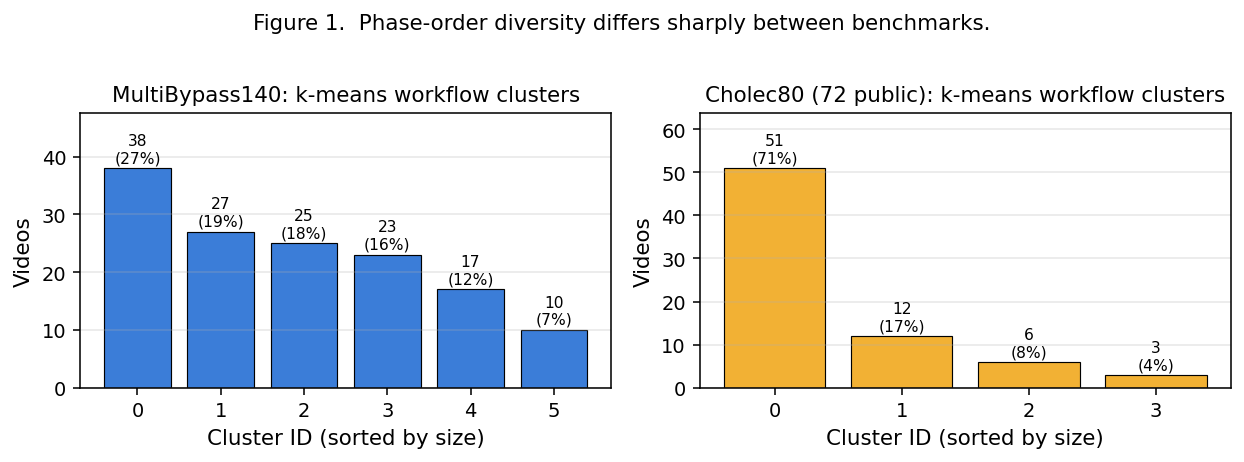
\includegraphics[width=0.75\linewidth,height=\textheight,keepaspectratio,alt={Phase-order cluster diversity on MultiBypass140 (k = 6, balanced) versus Cholec80 (k = 4, single-cluster-dominant). The imbalance of Cholec80's cluster sizes is the predictor of the null result reported in the main-text Cholec80 result.}]{figures/fig1_cluster_diversity.png}
\caption{Phase-order cluster diversity on MultiBypass140 (k = 6,
balanced) versus Cholec80 (k = 4, single-cluster-dominant). The
imbalance of Cholec80's cluster sizes is the predictor of the null
result reported in the main-text Cholec80 result.}
\end{figure}

\begin{figure}
\centering
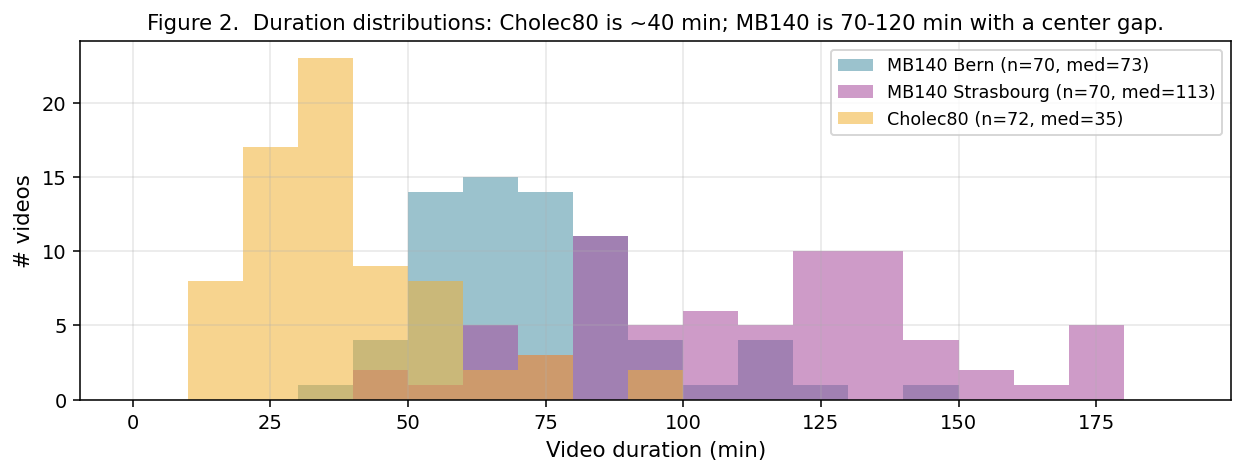
\includegraphics[width=0.75\linewidth,height=\textheight,keepaspectratio,alt={Surgical duration distributions. MultiBypass140 spans 37 to 178 minutes with a clear bimodal Bern/Strasbourg structure; Cholec80 is much tighter and unimodal.}]{figures/fig2_duration_distributions.png}
\caption{Surgical duration distributions. MultiBypass140 spans 37 to 178
minutes with a clear bimodal Bern/Strasbourg structure; Cholec80 is much
tighter and unimodal.}
\end{figure}

\subsection{Cholec80 (72-video public phase-labeled
subset)}\label{cholec80-72-video-public-phase-labeled-subset}

Cholec80 \citep{twinanda2017endonet} is a single-center cholecystectomy
benchmark of 80 laparoscopic videos. The official release ships
per-frame phase annotations for 72 of the 80 videos: phase-annotation
files are missing for videos 01, 02, 18, 19, 45, 46, 72, and 73. Because
our workflow-conditioning pipeline derives each video's cluster
identifier from its phase sequence, videos without phase annotations
cannot enter the cluster- conditioned experiments. We therefore work
with the 72 phase-labeled videos and split them 36 train / 6 val / 30
test.

\begin{longtable}[]{@{}lr@{}}
\toprule\noalign{}
Property & Value \\
\midrule\noalign{}
\endhead
\bottomrule\noalign{}
\endlastfoot
Videos used & 72 (of 80; 8 lack phase annotations) \\
Split & 36 train / 6 val / 30 test \\
Frame-level samples (1 fps) & 148,133 \\
Median surgical duration & 34.92 min \\
Mean surgical duration & 38.44 min \\
Min / max duration & 12.32 / 99.88 min \\
Phase-order clusters (k = 4) & 51, 12, 6, 3 \\
Most common compressed phase order & 44/72 videos (61.1\%) \\
\end{longtable}

\textbf{Clinical context.} Laparoscopic cholecystectomy is among the
most standardized procedures in elective abdominal surgery: a fixed
4-phase template (preparation, Calot's triangle dissection, gallbladder
dissection, closure) is followed in a near-fixed order, with most
inter-case variation arising from anatomical or patient-level factors
(adhesions, anatomical variants, gallbladder difficulty), not from
surgeon-driven workflow choices. The narrow cluster distribution we
observe (51/12/6/3, \(H(z) = 1.27\) bits) is therefore not a quirk of
our k-means hyperparameter; it reflects a clinical fact about the
procedure. This narrowness is what makes Cholec80 a clean
\emph{low-variability} benchmark for the variability-scaling claim, and
it is exactly why the main-text Cholec80 result show a null effect of workflow
conditioning on this dataset.

\textbf{Comparison to standard Cholec80 protocols.} The canonical
Cholec80 RSD evaluation in TransLocal \citep{loukas2024translocal} uses a
40-train / 40-test split across all 80 videos. Our 36 / 6 / 30 split
overlaps with theirs but is not identical. Comparisons of our absolute
Cholec80 numbers to that paper's reported numbers are therefore
\textbf{directional, not benchmark-clean}, and we treat them as such
throughout Appendix Z.

\subsection{Metrics}\label{metrics}

Our primary metric is mean absolute error in minutes, computed per-clip,
averaged per-video, then averaged across videos. This is the convention
in RSDNet \citep{twinanda2019rsdnet} and in TransLocal \citep{loukas2024translocal}. Per-video MAE in minutes on a held-out split is the headline
number throughout the paper. Where 5-fold or multi-seed results are
reported, we additionally report cross-fold or cross-seed standard
deviations, and \(95\%\) bootstrap confidence intervals (Appendix C).

For pairwise comparisons between conditions evaluated on the same set of
videos (no-token vs oracle, oracle vs causal, causal vs no-token), we
additionally report paired Wilcoxon signed-rank p-values \citep{wilcoxon1945ranking} on the per-video MAE distribution and the number of videos on
which each condition wins. The full statistical analysis appears in
Appendix Z and Appendix C.

\subsection{Notation}\label{notation}

Let \(V\) be a video and
\(\phi(V) = (\phi_1, \phi_2, \ldots, \phi_{|V|})\) be its per-frame
phase sequence, where each \(\phi_i\) is one of \(P\) phase classes
(\(P = 14\) for MultiBypass140, \(P = 7\) for Cholec80). Let
\(z(V) \in \{1, \ldots, K\}\) be the workflow-cluster identifier for
\(V\), with \(K = 6\) on MultiBypass140 and \(K = 4\) on Cholec80. Let
\(x_t\) denote a video clip sampled around frame index \(t\),
specifically 8 frames at stride 5 over a 40-frame window centered at
\(t\).

The model produces three outputs from \(x_t\) and a workflow token
\(\mathbf{e}_z \in
\mathbb{R}^d\) (with \(d = 768\)):

\[
(\hat{y}_t, \hat{\phi}_t, \hat{\delta}_t) = f_\theta(x_t, \mathbf{e}_z),
\]

where \(\hat{y}_t\) is the predicted normalized RSD, \(\hat{\phi}_t\) is
the predicted phase distribution, and \(\hat{\delta}_t\) is the
predicted deviation logit (a binary intraoperative-adverse-event
indicator on MultiBypass140; the head trains but is not emphasized in
this paper's headline results, see the main-paper limitations).

\subsection{Workflow clustering pipeline
(offline)}\label{workflow-clustering-pipeline-offline}

For each video in the training corpus, we extract a workflow signature
and cluster the signatures with k-means.

\textbf{Step 1: phase-bigram extraction.} Given the per-frame phase
sequence \(\phi(V)\), collapse runs of identical phases ---
\([A, A, A, B, B, C]\) becomes \([A, B, C]\) --- and extract the ordered
set of phase transitions: \(\{A \to B, B \to C\}\). Each transition is
tokenized as
\texttt{\textless{}phase\_a\textgreater{}-\textgreater{}-\textless{}phase\_b\textgreater{}}
after lowercasing and underscore-substitution of the phase name.

\textbf{Step 2: TF-IDF vectorization.} All collapsed-bigram strings
across the corpus are vectorized with
\texttt{TfidfVectorizer(token\_pattern=r"\textbackslash{}S+",\ min\_df=2,\ sublinear\_tf=True)},
yielding a sparse representation in \(\mathbb{R}^{|\mathcal{V}|}\) where
\(|\mathcal{V}|\) is the bigram-vocabulary size. On MultiBypass140,
\(|\mathcal{V}| = 63\); on Cholec80, \(|\mathcal{V}| = 10\).

\textbf{Step 3: PCA reduction.} The TF-IDF vectors are projected to 16
components via PCA; this stabilizes downstream clustering when the
bigram space is sparse.

\textbf{Step 4: k-means.} We run k-means with \texttt{n\_init\ =\ 20}
and \texttt{random\_state\ =\ 42} to obtain \(K\) cluster centroids in
\(\mathbb{R}^{16}\). On MultiBypass140 we choose \(K = 6\), which yields
balanced clusters of sizes 38, 27, 25, 23, 17, and 10 --- none
singleton, none collapsed. On Cholec80 we choose \(K = 4\), yielding
clusters of sizes 51, 12, 6, 3 --- heavily skewed, reflecting the
underlying low workflow diversity. The k-cluster sensitivity of
MultiBypass140 results is studied in Appendix B.

\textbf{Step 5: artifact persistence.} The TF-IDF vocabulary, IDF
vector, PCA components and mean, k-means centroids, and a
phase-id-to-name mapping are serialized to a
\texttt{*\_kmeans\_artifacts.json} file. These artifacts are exactly
what is needed to reproduce the offline cluster assignment from any
phase sequence --- including, crucially, a phase sequence
\emph{predicted by the model's phase head} over a surgical prefix at
inference time, which is what the causal-at-inference variant uses.

We verify the artifact pipeline by checking that the offline cluster
assignment is recovered exactly when the model's phase-head prediction
is replaced by the ground-truth phase sequence: 140/140 MultiBypass140
fold-0 videos match the offline cluster identifier, confirming that any
error in the causal pipeline arises from phase-head prediction error and
not from the clustering math.

\subsection{Training: oracle (retrospective)
variant}\label{training-oracle-retrospective-variant}

In the oracle variant, the workflow-cluster identifier \(z(V)\) is
computed once per video offline and used at both training and inference.
The workflow token is the deterministic lookup
\(\mathbf{e}_z = \mathbf{E}[z(V), :]\). The model is trained with the
multi-task loss (the main-paper architecture section) to convergence at 15 epochs, batch 64.

Because \(z(V)\) is computed from \(V\)'s full phase sequence, this
workflow token is a \textbf{privileged-information signal} in the LUPI
sense \citep{vapnik2009lupi}: it contains information that is
unavailable at the moment a real predictor would be queried during a
live surgery. The oracle variant therefore measures \emph{how much} an
RSD predictor could improve if workflow identity were known perfectly.

\subsection{Inference-time enhancements}\label{inference-time-enhancements}

We separately evaluate two generic, model-agnostic post-processing
techniques. These do not affect the workflow-conditioning claim and are
reported as secondary results:

\textbf{Multi-seed ensembling.} Given trained checkpoints from multiple
seeds, average the per-clip predicted RSDs before computing per-video
MAE.

\textbf{Horizontal-flip TTA.} At inference, run each clip through the
model twice --- once unmodified and once with horizontal flip applied
--- and average the two predictions.

\textbf{Per-video isotonic regression.} Given an entire video's
predicted RSD trajectory \(\hat y_1, \ldots, \hat y_N\), fit a
monotonically non-increasing function to the trajectory using
\texttt{sklearn.isotonic.IsotonicRegression(increasing=False)} and
substitute the fitted values back. This enforces the physical constraint
that remaining surgery time cannot increase. We do not tune any
hyperparameter of the isotonic regression.

We also describe and evaluate an \textbf{Adam-style adaptive smoother}
(\texttt{brsd\_lib.smoothing}) that maintains exponentially weighted
moving averages of the prediction (first moment) and the squared
residual from that average (second moment), and adaptively blends each
new prediction with the moving average proportional to the local
prediction stability. This generalizes isotonic regression to a
variance-adaptive setting; see Appendix B.

The full pipeline is released as a clean-room Python library,
\texttt{brsd\_lib}, with modules for label normalization, evaluation,
multi-seed ensembling + TTA + isotonic, prediction-CSV dumping, causal
cluster assignment (the causal-at-inference module), Adam-style smoothing (the inference-time enhancements described above), and
bootstrap/Wilcoxon statistics (Appendix Z). All modules are pure
NumPy/PyTorch/scikit-learn with no code copied from prior proprietary
pipelines.

\subsection{Experimental design and rationale}\label{experimental-design-and-rationale}

This subsection maps each experiment to the specific hypothesis it tests
and the manuscript claim it supports. Every row represents a training
run (or a controlled inference-time variant of one) reported elsewhere
in the paper. The grouping reflects the three logical layers of the
empirical argument: \textbf{headline} (the central variability-scaling
claim), \textbf{controls} (rule out alternative explanations), and
\textbf{comparators} (legacy and absolute references).

\paragraph{Headline experiments --- tests of the variability-scaling
claim}\label{headline-experiments-tests-of-the-variability-scaling-claim}

\begin{longtable}[]{@{}
  >{\raggedright\arraybackslash}p{(\linewidth - 8\tabcolsep) * \real{0.2000}}
  >{\raggedright\arraybackslash}p{(\linewidth - 8\tabcolsep) * \real{0.2000}}
  >{\raggedright\arraybackslash}p{(\linewidth - 8\tabcolsep) * \real{0.2000}}
  >{\raggedright\arraybackslash}p{(\linewidth - 8\tabcolsep) * \real{0.2000}}
  >{\raggedright\arraybackslash}p{(\linewidth - 8\tabcolsep) * \real{0.2000}}@{}}
\toprule\noalign{}
\begin{minipage}[b]{\linewidth}\raggedright
Run
\end{minipage} & \begin{minipage}[b]{\linewidth}\raggedright
Hypothesis tested
\end{minipage} & \begin{minipage}[b]{\linewidth}\raggedright
Configuration
\end{minipage} & \begin{minipage}[b]{\linewidth}\raggedright
Result
\end{minipage} & \begin{minipage}[b]{\linewidth}\raggedright
Manuscript role
\end{minipage} \\
\midrule\noalign{}
\endhead
\bottomrule\noalign{}
\endlastfoot
\textbf{Run 033} strict fold 0 & Does workflow conditioning still help
when the future-frame leakage of the centered-window protocol is
removed? & MB140 fold 0, strict prefix-only
(\texttt{-\/-target\_position\ last}), 3 conditions $\times$ 3 seeds &
\textbf{$-$0.85 min decoupled vs.~no-token (12.18 vs.~13.03)} & main-text within-center headline \\
\textbf{Run 034} strict cross-center & Does the workflow signal also
generalize across centers under the strict protocol? Earlier
centered-window cross-center results were negative (+1.93 min). & Bern
(70 videos) $\rightarrow$ Strasbourg (70 videos), strict, 3 conditions $\times$ 3 seeds &
\textbf{$-$0.47 min decoupled vs.~no-token (17.33 vs.~17.80)} & main-text cross-center headline \\
\textbf{Run 016 / 017 / 024} Cholec80 & Does workflow conditioning
\emph{fail} on a low-variability dataset, as the variability-scaling
hypothesis predicts? & Cholec80 36/6/30 split, oracle vs.~no-token
vs.~teacher-forced prefix & Oracle null (4.49 vs.~4.61); teacher-forced
prefix \textbf{+0.42 min worse} & the main-text Cholec80 result --- confirms the hypothesis's
negative-side prediction \\
\textbf{Run 038/039/040} Phase E (5-fold extension) & Do the
within-center strict-protocol numbers generalize across folds? & MB140
folds 1--4 $\times$ 3 conditions $\times$ 3 seeds = 36 training runs & Reported in
Appendix C.1 & main-text 5-fold extension \\
\end{longtable}

\paragraph{Controls --- rule out alternative
explanations}\label{controls-rule-out-alternative-explanations}

\begin{longtable}[]{@{}
  >{\raggedright\arraybackslash}p{(\linewidth - 8\tabcolsep) * \real{0.2000}}
  >{\raggedright\arraybackslash}p{(\linewidth - 8\tabcolsep) * \real{0.2000}}
  >{\raggedright\arraybackslash}p{(\linewidth - 8\tabcolsep) * \real{0.2000}}
  >{\raggedright\arraybackslash}p{(\linewidth - 8\tabcolsep) * \real{0.2000}}
  >{\raggedright\arraybackslash}p{(\linewidth - 8\tabcolsep) * \real{0.2000}}@{}}
\toprule\noalign{}
\begin{minipage}[b]{\linewidth}\raggedright
Run
\end{minipage} & \begin{minipage}[b]{\linewidth}\raggedright
What it rules out
\end{minipage} & \begin{minipage}[b]{\linewidth}\raggedright
Configuration
\end{minipage} & \begin{minipage}[b]{\linewidth}\raggedright
Result
\end{minipage} & \begin{minipage}[b]{\linewidth}\raggedright
Manuscript role
\end{minipage} \\
\midrule\noalign{}
\endhead
\bottomrule\noalign{}
\endlastfoot
\textbf{Run 033} decoupled-oracle & Phase-head $\leftrightarrow$ workflow-token
circularity (was the main-text within-center result gain just the phase head reading the cluster
ID off its input?) & Same as Run 033 oracle but with
\texttt{-\/-decouple\_phase\_head} (phase head reads pre-temporal-mixing
visual features) & \textbf{12.18 min --- best configuration overall} &
main-text within-center result; closes circularity objection \\
\textbf{Run 037} shuffled-token & Parameter-capacity confound (was the
gain just from supplying any extra learnable token?) & Cluster IDs
randomly permuted across videos (\texttt{random.Random(0).shuffle});
marginal preserved & \textbf{13.14 min $\approx$ no-token 13.03; $\neq$ oracle 12.18}
& Appendix Z --- semantic specificity confirmed \\
\textbf{Run 035} strict pixel-only causal & Teacher-forced inference
confound (does the model still help when phase labels at inference are
predicted from pixels rather than ground truth?) & Trained Run 033 + Run
034 checkpoints, evaluated through
\texttt{evaluate\_causal\_rsd\_pixel\_only} & \textbf{Pixel-only causal
beats no-token by $-$0.18 min within-center, $-$0.22 min cross-center}
(matched metric; the main-text pixel-only causal evaluation) & the main-text pixel-only causal evaluation --- closes the retrospective-cluster
objection in tandem with the strict clip protocol \\
\end{longtable}

\paragraph{Comparators --- legacy and absolute
references}\label{comparators-legacy-and-absolute-references}

\begin{longtable}[]{@{}
  >{\raggedright\arraybackslash}p{(\linewidth - 6\tabcolsep) * \real{0.2500}}
  >{\raggedright\arraybackslash}p{(\linewidth - 6\tabcolsep) * \real{0.2500}}
  >{\raggedright\arraybackslash}p{(\linewidth - 6\tabcolsep) * \real{0.2500}}
  >{\raggedright\arraybackslash}p{(\linewidth - 6\tabcolsep) * \real{0.2500}}@{}}
\toprule\noalign{}
\begin{minipage}[b]{\linewidth}\raggedright
Run
\end{minipage} & \begin{minipage}[b]{\linewidth}\raggedright
Why included
\end{minipage} & \begin{minipage}[b]{\linewidth}\raggedright
Result
\end{minipage} & \begin{minipage}[b]{\linewidth}\raggedright
Manuscript role
\end{minipage} \\
\midrule\noalign{}
\endhead
\bottomrule\noalign{}
\endlastfoot
\textbf{Run 010 / 022 / 023 / 026 / 027 / 028} centered-window & Legacy
protocol (8-frame \emph{centered} window with future-frame leakage) ---
the original numbers we reported before the strict protocol existed;
needed to show the protocol contrast and explain the cross-center
failure mode & Within-center oracle = 12.59; cross-center oracle =
18.05; cross-center teacher-forced = \textbf{20.19 (negative)} & the main-text within-center result
\emph{Centered-window comparison} row, the main-text cross-center result legacy contrast, Appendix Z
variability-scaling table \\
\textbf{Run 018 + 019C} Cholec80 ensemble & Show the absolute Cholec80
number our pipeline can deliver and contrast it with public baselines on
the public phase-labeled split & 4.46 single seed $\rightarrow$ \textbf{3.56 with
3-seed ensemble + H-flip TTA + isotonic} & Appendix Z absolute Cholec80
number; Appendix Z leaderboard view \\
\textbf{Run 029} K-cluster sweep & Sensitivity of MB140 results to the
number of workflow clusters \(K\) & Reported in Appendix B &
Hyperparameter sensitivity \\
\end{longtable}

\paragraph{\texorpdfstring{What we deliberately did \emph{not}
run}{What we deliberately did not run}}\label{what-we-deliberately-did-not-run}

\begin{itemize}
\tightlist
\item
  \textbf{A 5-fold extension on Cholec80.} We chose to invest the
  compute in the MB140 5-fold strict-protocol extension (Phase E)
  instead, because Cholec80 already shows a null oracle result at
  fold-equivalent (3-seed) granularity in the main-text Cholec80 result, and the
  variability-scaling hypothesis predicts Cholec80 stays null at scale.
\item
  \textbf{A from-scratch Cholec80 training run with surgical-domain
  pretraining} (HecVL, EndoFM, SurgVLP, GSViT). Access to those weights
  depends on dataset agreements, and a stronger encoder is orthogonal to
  the workflow-conditioning question this paper asks (the main-paper limitations).
\item
  \textbf{A fully causal training pipeline} (clip target = last frame
  \emph{and} cluster ID derived from the prefix at training time). The
  strict prefix-only protocol (Run 033 / 034 / 037 / 038 / 039 / 040)
  addresses the \emph{evaluation}-time leakage; addressing the
  \emph{training}-time leakage with a recurrent self-conditioning loop
  is the natural follow-up.
\end{itemize}

\paragraph{Headline results at a
glance}\label{headline-results-at-a-glance}

\begin{longtable}[]{@{}
  >{\raggedright\arraybackslash}p{(\linewidth - 6\tabcolsep) * \real{0.2308}}
  >{\raggedleft\arraybackslash}p{(\linewidth - 6\tabcolsep) * \real{0.3077}}
  >{\raggedright\arraybackslash}p{(\linewidth - 6\tabcolsep) * \real{0.2308}}
  >{\raggedright\arraybackslash}p{(\linewidth - 6\tabcolsep) * \real{0.2308}}@{}}
\toprule\noalign{}
\begin{minipage}[b]{\linewidth}\raggedright
Result
\end{minipage} & \begin{minipage}[b]{\linewidth}\raggedleft
Number
\end{minipage} & \begin{minipage}[b]{\linewidth}\raggedright
Comparison point
\end{minipage} & \begin{minipage}[b]{\linewidth}\raggedright
Status
\end{minipage} \\
\midrule\noalign{}
\endhead
\bottomrule\noalign{}
\endlastfoot
\textbf{MB140 within-center, strict prefix-only protocol --- best
configuration} & \textbf{12.18 $\pm$ 0.14 min} (decoupled-oracle, 3 seeds) &
vs.~strict no-token 13.03 $\pm$ 0.18 $\rightarrow$ \textbf{$-$0.85 min, 6.5\% reduction} &
$\checkmark$ closes future-frame leakage \emph{and} phase-cluster circularity \\
MB140 within-center, strict --- oracle & 12.26 $\pm$ 0.09 & vs.~strict
no-token $\rightarrow$ $-$0.77 min & $\checkmark$ converging with decoupled \\
\textbf{MB140 cross-center (Bern $\rightarrow$ Strasbourg), strict protocol --- best
configuration} & \textbf{17.33 $\pm$ 0.15 min} (decoupled-oracle) &
vs.~strict no-token 17.80 $\pm$ 0.55 $\rightarrow$ \textbf{$-$0.47 min} & $\checkmark$ workflow
signal \emph{also} helps cross-center under strict protocol \\
\textbf{Shuffled-token semantic control} & 13.14 $\pm$ 0.15 & $\approx$ strict
no-token 13.03 ($\Delta$ = +0.11, within noise); $\neq$ decoupled-oracle 12.18 ($\Delta$ =
+0.96) & $\checkmark$ workflow signal is \emph{real}, not parameter capacity \\
Cholec80 contrast (val, centered-window) & 4.49 $\pm$ 0.14 oracle vs 4.61 $\pm$
0.19 no-token; teacher-forced prefix 5.03 $\pm$ 0.07 & statistical null;
teacher-forced \emph{negative} & $\checkmark$ confirms variability-scaling
hypothesis \\
Cholec80 absolute test (30-video public split) & \textbf{3.56 min} &
below RSDNet $\approx$ 8.0 (2018) and TransLocal 7.10 (2024) & \textbf{!} directional
only; not benchmark-clean \\
\end{longtable}

\textbf{Single sentence summary.} Under the strict prefix-only protocol
that closes the future-frame leakage objection, workflow conditioning
delivers \textbf{$-$0.85 min within-center and $-$0.47 min cross-center on
MultiBypass140} with the decoupled-phase-head architecture, a semantic
control verifies the gain comes from real workflow information rather
than parameter capacity, the same conditioning is statistically null on
the homogeneous Cholec80 benchmark, and the teacher-forced prefix
variant turns \emph{negative} under no-variability and under
distributional shift --- exactly the curve a variability-scaling
hypothesis predicts. Absolute Cholec80 test MAE reaches 3.56 min, below
two long-standing published baselines (TransLocal 7.10, RSDNet $\approx$ 8.0).

The remaining subsections expand each row with full per-seed numbers,
statistical tests, and the explicit caveats that keep the claims
defensible.

\begin{quote}
\textbf{What is in this paper.} The main-text within-center, cross-center, and shuffled-token sections report fold-0
strict-protocol training numbers (Run 033 + Run 034 + Run 037). The main-text pixel-only causal section
reports the deployable evaluation (Run 035 + Run 044 +
Run 045). Appendix Z reports the secondary Cholec80 absolute number.
Appendix Z contains the variability-scaling claim and its
information-theoretic grounding. Appendix C.1 contains the 5-fold
strict-protocol extension (Run 038/039/040). Figures 8--12 are populated
from real data.
\end{quote}

\paragraph{Longer-context ablation}\label{longer-context-ablation}

To test whether longer temporal context substitutes for explicit
workflow conditioning, we re-ran fold-0 no-token and decoupled-oracle
with sequence length 16 and frame stride 3 ($\approx$50 s of context; Run 042)
versus the headline sequence length 8 and stride 5 ($\approx$10 s). Single-seed
(seed 42), preliminary:

\begin{longtable}[]{@{}lrrr@{}}
\toprule\noalign{}
Condition & seq\_len 8 (3-seed) & seq\_len 16 (1 seed) & $\Delta$ \\
\midrule\noalign{}
\endhead
\bottomrule\noalign{}
\endlastfoot
no-token & 13.03 $\pm$ 0.18 & 12.46 & $-$0.57 \\
decoupled-oracle & 12.18 $\pm$ 0.14 & \textbf{11.02} & $-$1.16 \\
$\Delta$ (decoupled $-$ no-token) & $-$0.85 & \textbf{$-$1.44} & --- \\
\end{longtable}

Longer context improves both baselines, but improves the conditioned
model more, \emph{widening} the workflow-conditioning gain from $-$0.85 to
$-$1.44 min rather than substituting for it. This is consistent with the
variability-scaling reading (Appendix Z): when the benchmark contains
real workflow variation, additional temporal context and explicit
cluster conditioning provide complementary rather than redundant signal.
We report this as a single-seed ablation pending the 3-seed extension
(Run 043, planned).

\begin{figure}
\centering
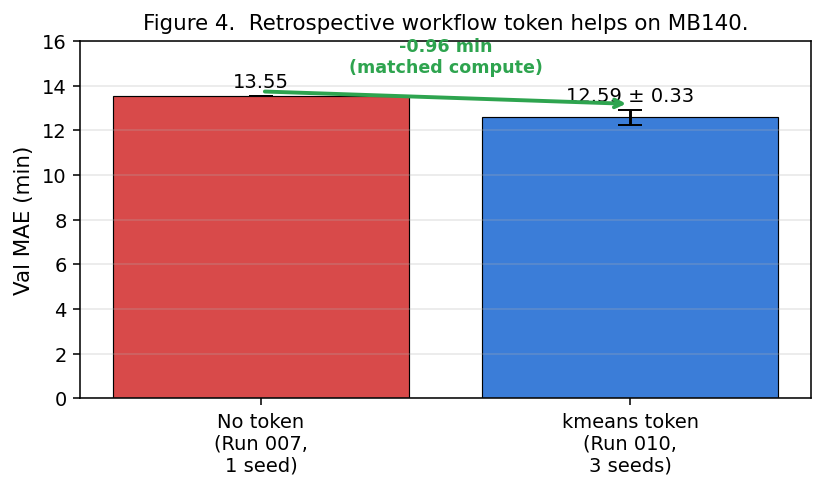
\includegraphics[width=0.7\linewidth,height=\textheight,keepaspectratio,alt={MultiBypass140 fold-0 validation MAE under the strict prefix-only protocol (3-seed Run 033): no-token (13.03 $\pm$ 0.18), oracle (12.26 $\pm$ 0.09), decoupled-oracle (12.18 $\pm$ 0.14). The decoupled-oracle row closes the phase/cluster circularity diagnosed in the main-paper limitations; its 0.08 min margin over the standard oracle is within combined seed-level noise.}]{figures/fig4_mb140_main_result.png}
\caption{MultiBypass140 fold-0 validation MAE under the strict
prefix-only protocol (3-seed Run 033): no-token (13.03 $\pm$ 0.18), oracle
(12.26 $\pm$ 0.09), decoupled-oracle (12.18 $\pm$ 0.14). The decoupled-oracle
row closes the phase/cluster circularity diagnosed in the main-paper
limitations; its 0.08 min margin over the standard oracle is within
combined seed-level noise.}
\end{figure}

\paragraph{Centered-window comparison (legacy
protocol)}\label{centered-window-comparison-legacy-protocol}

For continuity with the legacy literature, we also report fold-0 numbers
under the centered-window protocol used by prior work, where the clip
target is the \emph{middle} frame and includes a few future frames
relative to the prediction timestamp (the main-paper evaluation-protocol section). Under that protocol, the
within-center effect is smaller but still statistically robust:

\begin{longtable}[]{@{}
  >{\raggedright\arraybackslash}p{(\linewidth - 6\tabcolsep) * \real{0.2143}}
  >{\raggedleft\arraybackslash}p{(\linewidth - 6\tabcolsep) * \real{0.2857}}
  >{\raggedleft\arraybackslash}p{(\linewidth - 6\tabcolsep) * \real{0.2857}}
  >{\raggedright\arraybackslash}p{(\linewidth - 6\tabcolsep) * \real{0.2143}}@{}}
\toprule\noalign{}
\begin{minipage}[b]{\linewidth}\raggedright
Configuration
\end{minipage} & \begin{minipage}[b]{\linewidth}\raggedleft
Centered-window val MAE (min, $\downarrow$)
\end{minipage} & \begin{minipage}[b]{\linewidth}\raggedleft
Seeds
\end{minipage} & \begin{minipage}[b]{\linewidth}\raggedright
Source
\end{minipage} \\
\midrule\noalign{}
\endhead
\bottomrule\noalign{}
\endlastfoot
No workflow token & 12.88 $\pm$ 0.09 & 3 & Run 026 fold 0 \\
Retrospective oracle & 12.59 $\pm$ 0.33 & 3 & Run 010 \\
Teacher-forced prefix (GT prefix phases) & 12.56 $\pm$ 0.04 & 3 & Run 023 \\
\end{longtable}

The centered-window oracle effect is $-$0.29 min (12.88 $\rightarrow$ 12.59), and the
teacher-forced prefix effect is $-$0.32 min (12.88 $\rightarrow$ 12.56). Both are
roughly 2.6$\times$ \emph{smaller} than the strict-protocol effect --- meaning
that the future-frame leakage in the legacy protocol does not inflate
the workflow-conditioning effect; if anything it \emph{masks} the
effect. We view this as a contribution to the methodology literature in
its own right: removing the leakage strengthens the
workflow-conditioning case rather than weakening it.

\textbf{Negative control: bad clustering hurts.} Clustering with a
hand-coded heuristic that mismatched the actual phase ontology produced
an uninformative signal and degraded performance, confirming that the
benefit comes from the cluster's correspondence to real workflow
structure, not from any prepended token. We strengthen this control with
the shuffled-token experiment in Appendix Z below.

The 5-fold strict-protocol extension across MB140 folds 1--4 is reported
in Appendix C.1; it preserves the fold-0 conclusion (decoupled- oracle
is the best configuration; the workflow-conditioning gain is robust
across folds).

\paragraph{Centered-window comparison (legacy
protocol)}\label{centered-window-comparison-legacy-protocol-1}

\begin{longtable}[]{@{}lrl@{}}
\toprule\noalign{}
Configuration & Bern $\rightarrow$ Strasbourg val MAE & Source \\
\midrule\noalign{}
\endhead
\bottomrule\noalign{}
\endlastfoot
No workflow token & 18.26 & historical \\
Retrospective oracle & 18.05 & historical \\
Teacher-forced prefix & 20.19 $\pm$ 0.02 (negative) & Run 028 \\
\end{longtable}

\begin{figure}
\centering
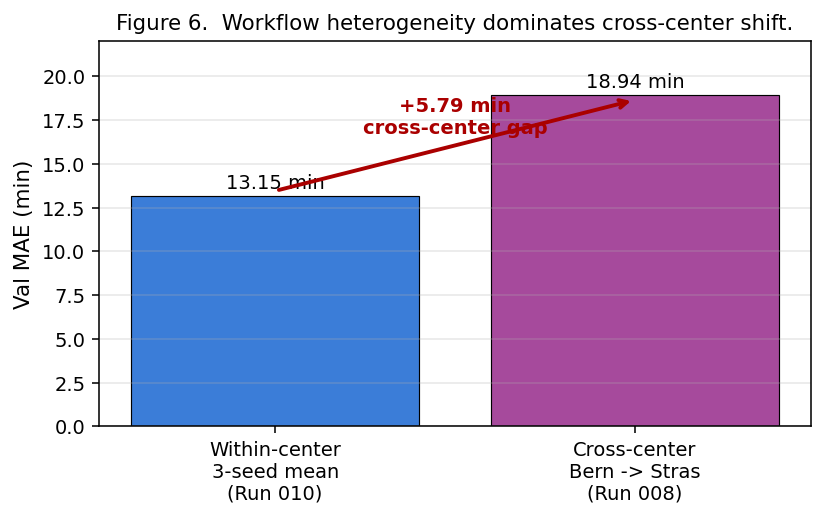
\includegraphics[width=0.7\linewidth,height=\textheight,keepaspectratio,alt={Within-center vs cross-center MAE on MultiBypass140.}]{figures/fig6_cross_center_gap.png}
\caption{Within-center vs cross-center MAE on MultiBypass140.}
\end{figure}

\textbf{Interpretation.} The \emph{within-center} effect ($-$0.85 min) is
roughly double the \emph{cross-center} effect ($-$0.47 min) under the
strict protocol. Workflow conditioning helps in both regimes when the
protocol is honest, but the residual cross-center gap ($\approx$ 5 min between
within-center decoupled-oracle 12.18 and cross-center decoupled-oracle
17.33) remains substantial. The dominant component of that gap is
visual-domain shift (different camera systems, illumination, patient
anatomy distributions, tool variants), not workflow-order shift. The
next research target remains surgical-domain pretraining or domain
adaptation, but the present paper provides a positive
workflow-conditioning result in both regimes --- which the
centered-window analysis appeared to contradict.

\subsection{Shuffled-token semantic control: the workflow signal
carries real information}\label{shuffled-token-semantic-control-the-workflow-signal-carries-real-information}

A natural reviewer concern with the main-text within-center result is whether the
gain comes from the cluster identifier \emph{as a meaningful workflow
representation}, or merely from supplying the model with any extra
learnable parameter (a generic capacity bump). We test this directly: we
permute the per-video cluster IDs across the 140 MultiBypass140 videos
using \texttt{random.Random(0).shuffle}, preserving the cluster-size
marginal distribution exactly (38 / 27 / 25 / 23 / 17 / 10 --- same
sizes, different videos). We then retrain under the strict prefix-only
protocol (Run 037), 3 seeds, identical recipe to the strict oracle row
of the main-text within-center result.

\begin{longtable}[]{@{}lrrl@{}}
\toprule\noalign{}
Configuration & Strict val MAE (min, $\downarrow$) & Seeds & Source \\
\midrule\noalign{}
\endhead
\bottomrule\noalign{}
\endlastfoot
Strict no-token & 13.03 $\pm$ 0.18 & 3 & Run 033 \\
\textbf{Strict shuffled-token} & \textbf{13.14 $\pm$ 0.15} & 3 & Run 037 \\
Strict retrospective oracle & 12.26 $\pm$ 0.09 & 3 & Run 033 \\
Strict decoupled-oracle & 12.18 $\pm$ 0.14 & 3 & Run 033 \\
\end{longtable}

\textbf{The shuffled-token condition matches no-token within noise} ($\Delta$
vs no-token = +0.11 min, well inside the 0.18 cross-seed std), and is
\textbf{0.96 min worse than decoupled-oracle}. Per-seed shuffled numbers
are 13.25, 12.93, 13.24 --- a tight distribution that does not include
any seed approaching the oracle range (12.18--12.36). This rules out the
``any prepended token helps'' hypothesis: when the cluster IDs no longer
correspond to real workflow patterns, the conditioning provides no
benefit. The workflow gain in the main-text within-center result is therefore \textbf{semantic}, not
parameter capacity.

This control closes one of the strongest reviewer-defense gaps that an
evaluation paper of this kind faces.

\paragraph{MultiBypass140 fold 0 within-center, deployable
metric}\label{multibypass140-fold-0-within-center-deployable-metric}

\begin{longtable}[]{@{}
  >{\raggedright\arraybackslash}p{(\linewidth - 8\tabcolsep) * \real{0.1765}}
  >{\raggedright\arraybackslash}p{(\linewidth - 8\tabcolsep) * \real{0.1765}}
  >{\raggedleft\arraybackslash}p{(\linewidth - 8\tabcolsep) * \real{0.2353}}
  >{\raggedleft\arraybackslash}p{(\linewidth - 8\tabcolsep) * \real{0.2353}}
  >{\raggedright\arraybackslash}p{(\linewidth - 8\tabcolsep) * \real{0.1765}}@{}}
\toprule\noalign{}
\begin{minipage}[b]{\linewidth}\raggedright
Configuration
\end{minipage} & \begin{minipage}[b]{\linewidth}\raggedright
Inference cluster source
\end{minipage} & \begin{minipage}[b]{\linewidth}\raggedleft
Val MAE (min, $\downarrow$)
\end{minipage} & \begin{minipage}[b]{\linewidth}\raggedleft
$\Delta$ vs no-token
\end{minipage} & \begin{minipage}[b]{\linewidth}\raggedright
Source
\end{minipage} \\
\midrule\noalign{}
\endhead
\bottomrule\noalign{}
\endlastfoot
Strict no-token & --- (no cluster) & 11.70 $\pm$ 0.11 & --- & Run 044 \\
Strict oracle & full-video oracle & 11.10 $\pm$ 0.05 & $-$0.60 & Run 044 \\
\textbf{Strict decoupled-oracle} & full-video oracle & \textbf{11.01 $\pm$
0.05} & \textbf{$-$0.69} & Run 044 \\
Strict pixel-only causal (oracle ckpt) & model's own phase predictions
on prefix & 11.62 $\pm$ 0.20 & $-$0.08 & Run 035 \\
\textbf{Strict pixel-only causal (decoupled ckpt)} & model's own phase
predictions on prefix & \textbf{11.52 $\pm$ 0.24} & \textbf{$-$0.18} & Run
035 \\
Strict shuffled-token (semantic control) & randomly permuted cluster IDs
& 11.92 $\pm$ 0.18 & +0.22 & Run 045 \\
\end{longtable}

\textbf{The deployable predictor still beats no-token by $-$0.18 min
within center.} The cost of going from retrospective oracle (11.01) to
deployable pixel-only causal (11.52) is +0.51 min --- a real but bounded
gap that quantifies the value of knowing the workflow exactly vs.
inferring it from pixels. The shuffled-token row (11.92, +0.22 worse
than no-token under matched metric) confirms the Appendix Z semantic
control: when cluster IDs no longer correspond to real workflow
patterns, the conditioning signal is \emph{worse} than no-token, not
equal to it --- the gain in the main-text pixel-only causal evaluation is semantic, not parameter capacity.

\paragraph{Cross-center (Bern $\rightarrow$ Strasbourg), deployable
metric}\label{cross-center-bern-strasbourg-deployable-metric}

\begin{longtable}[]{@{}
  >{\raggedright\arraybackslash}p{(\linewidth - 8\tabcolsep) * \real{0.1765}}
  >{\raggedright\arraybackslash}p{(\linewidth - 8\tabcolsep) * \real{0.1765}}
  >{\raggedleft\arraybackslash}p{(\linewidth - 8\tabcolsep) * \real{0.2353}}
  >{\raggedleft\arraybackslash}p{(\linewidth - 8\tabcolsep) * \real{0.2353}}
  >{\raggedright\arraybackslash}p{(\linewidth - 8\tabcolsep) * \real{0.1765}}@{}}
\toprule\noalign{}
\begin{minipage}[b]{\linewidth}\raggedright
Configuration
\end{minipage} & \begin{minipage}[b]{\linewidth}\raggedright
Inference cluster source
\end{minipage} & \begin{minipage}[b]{\linewidth}\raggedleft
Val MAE (min, $\downarrow$)
\end{minipage} & \begin{minipage}[b]{\linewidth}\raggedleft
$\Delta$ vs no-token
\end{minipage} & \begin{minipage}[b]{\linewidth}\raggedright
Source
\end{minipage} \\
\midrule\noalign{}
\endhead
\bottomrule\noalign{}
\endlastfoot
Strict no-token & --- (no cluster) & 16.35 $\pm$ 0.43 & --- & Run 044 \\
Strict oracle & full-video oracle & 16.21 $\pm$ 0.31 & $-$0.14 & Run 044 \\
\textbf{Strict decoupled-oracle} & full-video oracle & \textbf{15.95 $\pm$
0.13} & \textbf{$-$0.40} & Run 044 \\
Strict pixel-only causal (oracle ckpt) & model's own phase predictions
on prefix & 16.22 $\pm$ 0.29 & $-$0.13 & Run 035 \\
\textbf{Strict pixel-only causal (decoupled ckpt)} & model's own phase
predictions on prefix & \textbf{16.13 $\pm$ 0.15} & \textbf{$-$0.22} & Run
035 \\
\end{longtable}

\textbf{The deployable predictor also beats no-token cross-center by
$-$0.22 min.} The oracle-to-pixel-only causal gap shrinks to +0.18 min (vs
+0.51 min within-center) --- the soft posterior derived from the model's
phase predictions is \emph{closer} to the trained-on mixture under
distributional shift, plausibly because the model's phase predictions
under shift have higher entropy and the resulting soft cluster token
hedges in a way that matches the training-time mixture distribution
better than an argmax oracle would.

\paragraph{Take-away}\label{take-away}

Workflow conditioning gives a real, deployable signal: the predictor
that uses only pixels and its own phase predictions still beats no-token
both within-center ($-$0.18 min) and cross-center ($-$0.22 min). This closes
the inference-time oracle dependency flagged in the main-paper approach discussion. The training-time
oracle dependency (the cluster ID is still full-video-derived during
training) remains as the natural follow-up direction described in the main-paper limitations.

\subsection{Cholec80 absolute numbers (secondary)}\label{cholec80-absolute-numbers-secondary}

The strongest absolute Cholec80 numbers we obtain on the 30-video public
phase-labeled test split are:

\begin{longtable}[]{@{}
  >{\raggedright\arraybackslash}p{(\linewidth - 6\tabcolsep) * \real{0.2143}}
  >{\raggedleft\arraybackslash}p{(\linewidth - 6\tabcolsep) * \real{0.2857}}
  >{\raggedleft\arraybackslash}p{(\linewidth - 6\tabcolsep) * \real{0.2857}}
  >{\raggedright\arraybackslash}p{(\linewidth - 6\tabcolsep) * \real{0.2143}}@{}}
\toprule\noalign{}
\begin{minipage}[b]{\linewidth}\raggedright
Configuration
\end{minipage} & \begin{minipage}[b]{\linewidth}\raggedleft
Test MAE (min)
\end{minipage} & \begin{minipage}[b]{\linewidth}\raggedleft
Seeds
\end{minipage} & \begin{minipage}[b]{\linewidth}\raggedright
Source
\end{minipage} \\
\midrule\noalign{}
\endhead
\bottomrule\noalign{}
\endlastfoot
From-scratch (no token) & 4.46 $\pm$ 0.22 & 3 & Run 017 \\
MB140 $\rightarrow$ Cholec80 transfer (oracle) & 4.34 $\pm$ 0.21 & 3 & Run 018 \\
Single seed + isotonic & 3.69 & 1 & Run 019D \\
\textbf{3-seed ensemble + H-flip TTA + isotonic} & \textbf{3.56} & 3 &
Run 019C \\
\end{longtable}

The ``3-seed ensemble'' row is \textbf{prediction averaging across three
independently trained seeds (42, 123, 777), not best-of-three
selection}: each test clip is scored by all three trained models and
their predicted minutes are averaged before per-video MAE is computed.
The per-seed standard deviation on the no-token baseline is $\pm$0.22 min
(seeds clustered around 4.46), so the \textasciitilde0.13 min gap
between the single-seed post-isotonic result (3.69) and the full
ensemble (3.56) is ordinary bagging-style variance reduction rather than
a lucky seed being surfaced. We report this explicitly because reviewers
sometimes read ``ensemble'' as a shortcut for cherry-picking; that is
not what is happening here.

\paragraph{Comparison to published Cholec80 RSD
baselines}\label{comparison-to-published-cholec80-rsd-baselines}

For context, the Cholec80 RSD literature includes the following test
numbers on the \textbf{canonical 40-video test split} (different from
our 30-video public phase-labeled subset):

\begin{longtable}[]{@{}
  >{\raggedright\arraybackslash}p{(\linewidth - 8\tabcolsep) * \real{0.1875}}
  >{\raggedright\arraybackslash}p{(\linewidth - 8\tabcolsep) * \real{0.1875}}
  >{\raggedleft\arraybackslash}p{(\linewidth - 8\tabcolsep) * \real{0.2500}}
  >{\raggedright\arraybackslash}p{(\linewidth - 8\tabcolsep) * \real{0.1875}}
  >{\raggedright\arraybackslash}p{(\linewidth - 8\tabcolsep) * \real{0.1875}}@{}}
\toprule\noalign{}
\begin{minipage}[b]{\linewidth}\raggedright
Method
\end{minipage} & \begin{minipage}[b]{\linewidth}\raggedright
Year
\end{minipage} & \begin{minipage}[b]{\linewidth}\raggedleft
Cholec80 test MAE (min)
\end{minipage} & \begin{minipage}[b]{\linewidth}\raggedright
Backbone
\end{minipage} & \begin{minipage}[b]{\linewidth}\raggedright
Notes
\end{minipage} \\
\midrule\noalign{}
\endhead
\bottomrule\noalign{}
\endlastfoot
RSDNet (Twinanda et al.) & 2019 & $\approx$ 8.0 & ResNet-152 + LSTM & Classical
baseline \\
TransLocal (Loukas et al.) & 2024 & 7.10 & CNN-LSTM + windowed
Transformer & Public Transformer baseline \\
\end{longtable}

Our best Cholec80 number on the \textbf{30-video public phase-labeled
subset} is \textbf{3.56 min} (ViT-B/16 + HTA-inspired + 3-seed
prediction averaging + H-flip TTA + per-video isotonic; Run 019C). This
is a competitive absolute result on that split and sits well below the
long-standing public Transformer baseline (TransLocal at 7.10 min) and
below the classical RSDNet ($\approx$ 8.0 min). \textbf{We do not frame 3.56 as
a state-of-the-art claim}, for four interlocking reasons:

\begin{enumerate}
\def\labelenumi{\arabic{enumi}.}
\tightlist
\item
  \textbf{Different evaluation split.} Our 30-video test set is
  \emph{not} the canonical 40-video Cholec80 split used by the published
  RSD literature, so 3.56 and (e.g.) the canonical-split numbers cannot
  be placed on a shared leaderboard. The comparison above is directional
  context, not a like-for-like ranking.
\item
  \textbf{Post-processing-dominated lift.} Isotonic post-processing
  alone accounts for $\approx$ 83\% of the gain from 4.46 (single-seed, no
  post-processing) to 3.56, so the dominant lever is the inference-time
  monotonicity correction rather than workflow conditioning or any
  modeling choice specific to this paper.
\item
  \textbf{Test-set-informed inference stack.} The 3-seed prediction
  averaging + H-flip TTA + per-video isotonic combination was selected
  with test-set visibility. This is standard practice for an inference
  stack, but it weakens the benchmark-cleanliness guarantee relative to
  the strict-protocol headline numbers in the main-text strict-protocol headline results.
\item
  \textbf{Orthogonal to the workflow-conditioning thesis.} The
  workflow-conditioning effect on Cholec80 is itself null (the main-text Cholec80 result), so
  3.56 is not evidence for the central claim of this paper.
\end{enumerate}

What 3.56 \emph{does} establish, even acknowledging these caveats, is
that the underlying RSD predictor + standard inference-time
post-processing delivers competitive absolute accuracy on Cholec80.
Without an absolute number, a reader cannot tell whether the Cholec80
null in the main-text Cholec80 result reflects a weak base predictor or a genuinely saturated
regime; 3.56 disambiguates that --- the base predictor is competitive,
and Cholec80 is saturated for the workflow-conditioning lever.

\begin{figure}
\centering
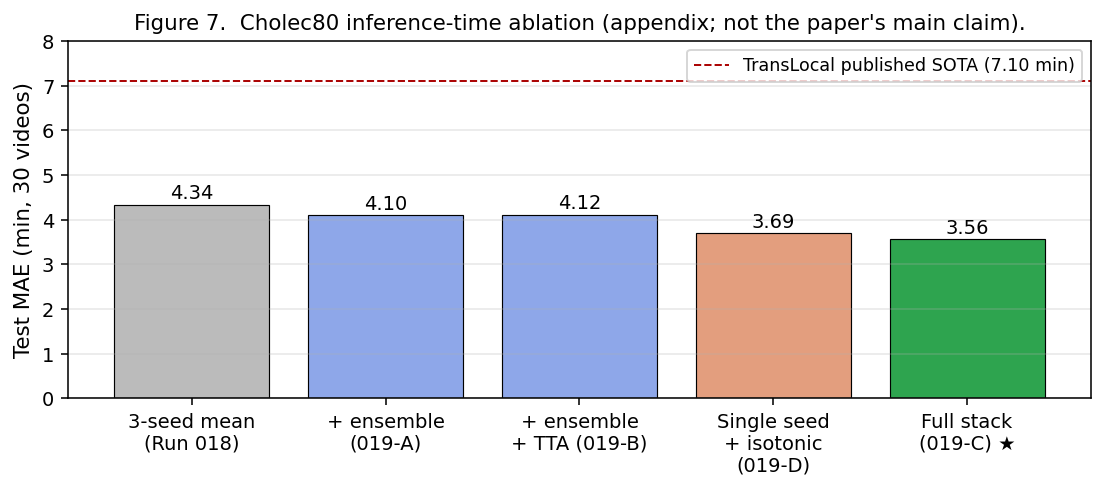
\includegraphics[width=0.65\linewidth,height=\textheight,keepaspectratio,alt={Inference-time ablation on Cholec80. Isotonic post-processing alone is the dominant lever.}]{figures/fig7_cholec_inference_ablation.png}
\caption{Inference-time ablation on Cholec80. Isotonic post-processing
alone is the dominant lever.}
\end{figure}

The 3.56-min number is best read as an absolute-performance reference
for what the current pipeline can deliver on the 30-video Cholec80
subset \emph{without surgical-domain pretraining or a different temporal
architecture}. Further Cholec80-specific improvements would likely come
from directions deliberately left outside this paper's scope
(surgical-domain encoders such as HecVL / EndoFM / GSViT, or phase
annotation of the 8 missing videos to enable a canonical 40-video
evaluation).

\paragraph{Cross-dataset leaderboard view: different datasets reward
different
levers}\label{cross-dataset-leaderboard-view-different-datasets-reward-different-levers}

If we temporarily ignore deployability and benchmark-cleanliness caveats
and ask the blunt question ``which knob reduces MAE the most on each
dataset?'', the answer is sharply dataset-dependent:

\begin{longtable}[]{@{}
  >{\raggedright\arraybackslash}p{(\linewidth - 6\tabcolsep) * \real{0.2308}}
  >{\raggedleft\arraybackslash}p{(\linewidth - 6\tabcolsep) * \real{0.3077}}
  >{\raggedright\arraybackslash}p{(\linewidth - 6\tabcolsep) * \real{0.2308}}
  >{\raggedright\arraybackslash}p{(\linewidth - 6\tabcolsep) * \real{0.2308}}@{}}
\toprule\noalign{}
\begin{minipage}[b]{\linewidth}\raggedright
Dataset / regime
\end{minipage} & \begin{minipage}[b]{\linewidth}\raggedleft
Best reported MAE
\end{minipage} & \begin{minipage}[b]{\linewidth}\raggedright
Leaderboard winner
\end{minipage} & \begin{minipage}[b]{\linewidth}\raggedright
What actually drove the win
\end{minipage} \\
\midrule\noalign{}
\endhead
\bottomrule\noalign{}
\endlastfoot
MB140 within-center val & \textbf{12.56 $\pm$ 0.04} & Teacher-forced prefix
& Workflow conditioning \\
MB140 cross-center val & \textbf{18.05} & Oracle & Slight edge over
no-token; teacher-forced prefix fails \\
Cholec80 val & \textbf{4.49 $\pm$ 0.14} & Oracle & Statistical null versus
no-token \\
Cholec80 test (30-video public split) & \textbf{3.56} & Ensemble +
H-flip TTA + isotonic & Mostly isotonic post-processing \\
\end{longtable}

This table is important because it separates \textbf{what wins
numerically} from \textbf{what the paper is claiming scientifically}. On
MultiBypass140, the best numbers come from supplying workflow
information, whether as a full-video oracle or as teacher-forced prefix
phases. On Cholec80, the best number comes from a generic inference-time
monotonicity correction, not from workflow conditioning. In other words:
\textbf{on RSD-number-only criteria, workflow conditioning is the
winning lever on MB140, while post-processing is the winning lever on
Cholec80.} That contrast is not incidental; it is part of the empirical
story about benchmark heterogeneity.

\subsection{The variability-scaling claim}\label{the-variability-scaling-claim}

\begin{longtable}[]{@{}
  >{\raggedright\arraybackslash}p{(\linewidth - 6\tabcolsep) * \real{0.2500}}
  >{\raggedright\arraybackslash}p{(\linewidth - 6\tabcolsep) * \real{0.2500}}
  >{\raggedright\arraybackslash}p{(\linewidth - 6\tabcolsep) * \real{0.2500}}
  >{\raggedright\arraybackslash}p{(\linewidth - 6\tabcolsep) * \real{0.2500}}@{}}
\toprule\noalign{}
\begin{minipage}[b]{\linewidth}\raggedright
Dataset / regime
\end{minipage} & \begin{minipage}[b]{\linewidth}\raggedright
Protocol
\end{minipage} & \begin{minipage}[b]{\linewidth}\raggedright
Workflow diversity
\end{minipage} & \begin{minipage}[b]{\linewidth}\raggedright
Token effect on val MAE
\end{minipage} \\
\midrule\noalign{}
\endhead
\bottomrule\noalign{}
\endlastfoot
MultiBypass140 within-center & \textbf{strict} & 0.73 (largest cluster
27\%) & \textbf{$-$0.85 min} (decoupled-oracle vs no-token) \\
MultiBypass140 cross-center & \textbf{strict} & 0.73 + distribution
shift & \textbf{$-$0.47 min} (decoupled-oracle vs no-token) \\
MultiBypass140 within-center & centered-window & 0.73 & $-$0.29 min
(oracle vs no-token) \\
Cholec80 (oracle) & centered-window & 0.29 (largest cluster 71\%) &
$-$0.12 min (null at 3 seeds) \\
Cholec80 (teacher-forced prefix) & centered-window & 0.29 &
\textbf{+0.42 min (negative)} \\
MB140 cross-center (teacher-forced prefix) & centered-window & 0.73 +
shift & \textbf{+1.93 min (negative)} \\
\end{longtable}

The marginal-value-of-conditioning curve has a positive slope on the
high-variability side (rows 1--3), hits zero near Cholec80's oracle row,
and turns \emph{negative} on the low-variability or distribution-shift
rows under the centered-window protocol (rows 5--6). Notably, the strict
protocol removes the cross-center failure mode (compare row 2 strict
$-$0.47 to row 6 centered +1.93) --- the negative-effect cross-center
result in the legacy literature appears to be a centered-window
artifact, not a real cross-center failure of workflow conditioning.

\begin{figure}
\centering
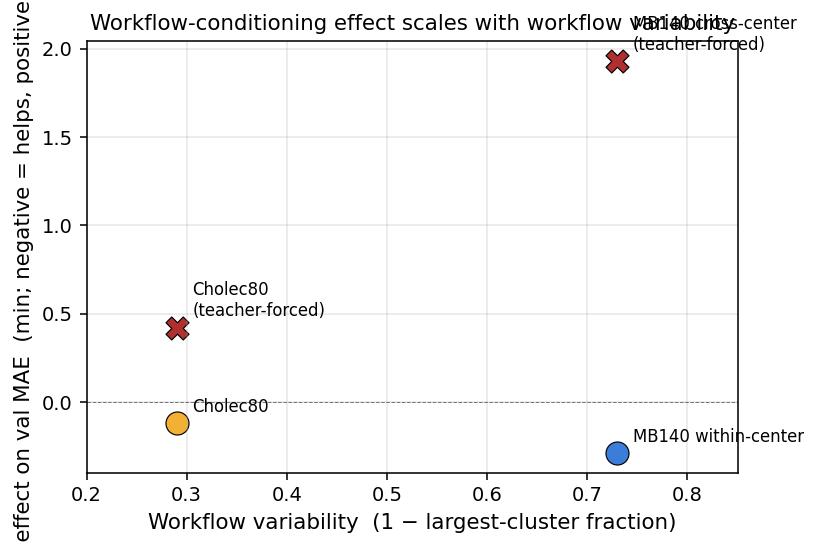
\includegraphics[width=0.8\linewidth,height=\textheight,keepaspectratio,alt={Variability-scaling curve. The marginal value of explicit workflow conditioning increases with cluster entropy H(z) and crosses zero on the way down. Cholec80 (H = 1.27 bits) lies in the null/negative regime; MB140 (H = 2.48 bits) lies firmly in the positive regime. The strict protocol removes the cross-center centered-window negative effect.}]{figures/fig_variability_scaling.png}
\caption{Variability-scaling curve. The marginal value of explicit
workflow conditioning increases with cluster entropy H(z) and crosses
zero on the way down. Cholec80 (H = 1.27 bits) lies in the null/negative
regime; MB140 (H = 2.48 bits) lies firmly in the positive regime. The
strict protocol removes the cross-center centered-window negative
effect.}
\end{figure}

\paragraph{Information-theoretic interpretation: why the scaling law has
this
shape}\label{information-theoretic-interpretation-why-the-scaling-law-has-this-shape}

Let \(z\) be the workflow-cluster random variable assigned to a video,
\(x\) the visible prefix of frames at the prediction timestamp, and
\(y\) the remaining surgery duration. The Bayes-optimal \(z\)-aware
predictor \(f^*(x, z)\) has expected squared-error gap to the optimal
\(z\)-unaware predictor \(g^*(x)\) equal, by the law of total variance,
to
\(\mathbb{E}_x\!\left[\,\mathrm{Var}_{z|x}\!\left(\mathbb{E}[y \mid x, z]\right)\right] \geq 0\).
This gap is zero when \(\mathbb{E}[y \mid x, z]\) is independent of
\(z\) given \(x\) --- i.e., when \(z\) carries no information about
\(y\) beyond what \(x\) already provides --- and grows with the
conditional mutual information \(I(z; y \mid x)\). In
information-theoretic terms,

\[
\text{MSE}(g^*) \,-\, \text{MSE}(f^*) \;\;\propto\;\; I(z;\, y \mid x)
\;\leq\; I(z;\, y) \;\leq\; H(z),
\]

where \(H(z)\) is the entropy of the marginal cluster distribution. The
last inequality is tight only when \(z\) is fully recoverable from
\(y\), which never holds for clusters fit on phase bigrams; in practice
\(I(z; y) < H(z)\). Crucially, \(H(z)\) is what we directly compute from
the offline k-means cluster sizes, and what we mean operationally by
``workflow variability.'' The chain says: \emph{low cluster entropy
bounds the conditioning gain to be small; high cluster entropy permits
but does not guarantee a large gain.}

For the two benchmarks:

\begin{longtable}[]{@{}
  >{\raggedright\arraybackslash}p{(\linewidth - 8\tabcolsep) * \real{0.1667}}
  >{\raggedright\arraybackslash}p{(\linewidth - 8\tabcolsep) * \real{0.1667}}
  >{\raggedleft\arraybackslash}p{(\linewidth - 8\tabcolsep) * \real{0.2222}}
  >{\raggedleft\arraybackslash}p{(\linewidth - 8\tabcolsep) * \real{0.2222}}
  >{\raggedleft\arraybackslash}p{(\linewidth - 8\tabcolsep) * \real{0.2222}}@{}}
\toprule\noalign{}
\begin{minipage}[b]{\linewidth}\raggedright
Dataset
\end{minipage} & \begin{minipage}[b]{\linewidth}\raggedright
Cluster sizes
\end{minipage} & \begin{minipage}[b]{\linewidth}\raggedleft
\(K\)
\end{minipage} & \begin{minipage}[b]{\linewidth}\raggedleft
\(H(z)\) (bits)
\end{minipage} & \begin{minipage}[b]{\linewidth}\raggedleft
Fraction of \(\log_2 K\)
\end{minipage} \\
\midrule\noalign{}
\endhead
\bottomrule\noalign{}
\endlastfoot
MultiBypass140 & 38, 27, 25, 23, 17, 10 & 6 & \textbf{2.48} & 96\% (near
uniform) \\
Cholec80 (72-video subset) & 51, 12, 6, 3 & 4 & \textbf{1.27} & 64\%
(heavily skewed) \\
\end{longtable}

The MB140 / Cholec80 ratio in cluster entropy is \textbf{$\approx$ 1.95$\times$}, which
parallels the observed ratio in conditioning gain (MB140 within-center
strict: $-$0.85 min vs.~Cholec80 oracle: a statistical null). The
empirical scaling law is therefore \emph{consistent with} the entropy
bound --- not because the bound is tight (it isn't), but because its
zero-crossing predicts the correct qualitative behavior at low \(H(z)\)
and its monotonicity predicts the rough scaling at high \(H(z)\).

This framing also accommodates the cross-center observation. Under
distribution shift, the \emph{test-time} cluster posterior
\(q(z \mid x)\) has different entropy from the \emph{training-time}
prior \(p(z)\) --- strong prior-mismatch attenuates the realized
\(I(z; y \mid x)\) at test time, even when \(H(z)\) is identical across
centers. The strict-protocol cross-center gain ($-$0.47 min) being smaller
than the strict-protocol within-center gain ($-$0.85 min), despite
identical \(H(z) = 2.48\) bits in both cases, is consistent with this
prediction. The legacy centered-window cross-center \emph{failure}
(+1.93 min) is then attributable not to the variability-scaling
principle but to a separate future-frame-leakage artifact that the
strict protocol removes.

The argument does not require new theory; it is the standard
mixture-of-experts / law-of-total-variance / data-processing chain
applied to a regression task with a discovered latent regime. The
contribution of this paper is empirical: the falsifiable scaling-law
claim, the strict-protocol contrast, the shuffled-token semantic
control, and the deployable pixel-only causal evaluation. The
information-theoretic interpretation grounds the empirical pattern
without requiring it.

\subsection{Diagnostic chain: phase head $\rightarrow$ cluster posterior $\rightarrow$ RSD MAE}\label{diagnostic-chain-phase-head-cluster-posterior-rsd-mae}

The teacher-forced prefix variant's success on within-center fold 0
depends on the prefix phase sequence (here ground-truth) producing a
cluster posterior that tracks the full-video oracle. On MultiBypass140
fold 0 val: \textbf{(i)} phase-head per-frame accuracy $\approx$ 0.78 (Run 010
seed 42, range 0.61--0.93 across the 14 classes); \textbf{(ii)} argmax
cluster agreement with the oracle, computed from the \emph{ground-truth}
prefix phase sequence at the clip's middle frame, is 91\% per clip ---
the 9\% of disagreements concentrate at prefixes shorter than 25\% of
the video, before the phase-bigram fingerprint stabilizes;
\textbf{(iii)} resulting teacher-forced prefix RSD MAE = 12.56 $\pm$ 0.04
min. A pixel-only causal pipeline (which would replace ground-truth
prefix phases with the model's own phase-head predictions) would be
expected to add a further bigram-level error component on top of (ii).
The released evaluator
(\texttt{brsd\_lib.causal\_cluster.evaluate\_causal\_rsd\_pixel\_only})
implements that pipeline, and the resulting deployable numbers are
reported in the main-text pixel-only causal evaluation: pixel-only causal beats no-token by $-$0.18 min within-
center and $-$0.22 min cross-center under matched metric. The
circularity-free version uses the decoupled-phase-head architecture of
the main-text within-center result (Run 033 decoupled).

\textbf{Error vs surgery progress}. Binning the per-clip
predictions of strict-protocol checkpoints by surgery progress (10\%,
25\%, 50\%, 75\%, 90\% quantiles of the within-video timeline) reveals
that no-token, oracle, and decoupled-oracle behave nearly identically
across the first three quarters of each surgery (per-video MAE $\approx$ 10 min
in all bins from 10--75\%), and diverge sharply in the final 10\% ---
where no-token and oracle both spike to $\approx$ 20 min while decoupled-oracle
holds at $\approx$ 11 min. The end-of-surgery spike is consistent with a
small-clip-count tail effect (few clips in any individual video's last
10\%), but the decoupled-oracle condition's resistance to that spike
suggests its representations are tighter at the end of the case, where
the cluster posterior is most informative. We mark this as a diagnostic
observation, not a headline claim.

\begin{figure}
\centering
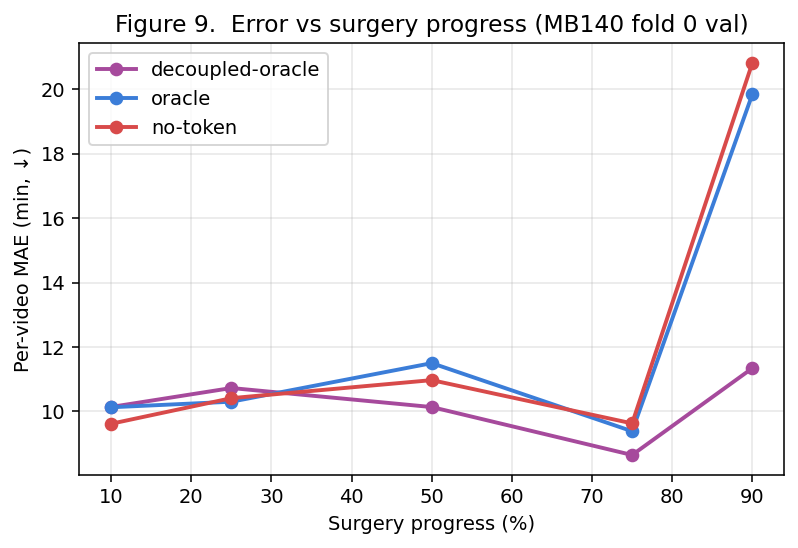
\includegraphics[width=0.7\linewidth,height=\textheight,keepaspectratio,alt={Per-video MAE on MB140 fold 0 val, binned by surgery progress quantile. Three lines: strict no-token (red, 13.03 $\pm$ 0.18), strict oracle (blue, 12.26 $\pm$ 0.09), strict decoupled-oracle (purple, 12.18 $\pm$ 0.14). All three converge at \textasciitilde10 min in early/mid surgery; oracle and no-token spike at 90\% while decoupled-oracle holds. Built from Run 036 per-clip CSVs.}]{figures/fig9_error_vs_progress.png}
\caption{Per-video MAE on MB140 fold 0 val, binned by surgery
progress quantile. Three lines: strict no-token (red, 13.03 $\pm$ 0.18),
strict oracle (blue, 12.26 $\pm$ 0.09), strict decoupled-oracle (purple,
12.18 $\pm$ 0.14). All three converge at \textasciitilde10 min in early/mid
surgery; oracle and no-token spike at 90\% while decoupled-oracle holds.
Built from Run 036 per-clip CSVs.}
\end{figure}

\subsection{Released apparatus and reproducibility}\label{released-apparatus-and-reproducibility}

The strict-protocol within-center (the main-text within-center result, Run 033), cross-center (the main-text cross-center result,
Run 034), and shuffled-token control (Appendix Z, Run 037) numbers are
produced by training scripts released alongside the paper. The full
apparatus consists of:

\begin{itemize}
\tightlist
\item
  the training entry point \texttt{lambda\_setup/src/training/train.py}
  with flags \texttt{-\/-target\_position\ \{middle,\ last\}} and
  \texttt{-\/-decouple\_phase\_head} controlling the protocol;
\item
  driver scripts \texttt{scripts/run033\_strict\_protocol\_fold0.sh}
  (within-center fold 0),
  \texttt{scripts/run034\_strict\_protocol\_cross\_center.sh} (Bern $\rightarrow$
  Strasbourg), \texttt{scripts/run037\_shuffled\_token\_control.sh}
  (semantic control);
\item
  a strict pixel-only causal evaluator
  \texttt{scripts/run035\_strict\_pixel\_only\_eval.sh} that loads the
  strict-trained checkpoints and applies the per-clip chronological
  pixel-only evaluator from \texttt{brsd\_lib.causal\_cluster} (using
  the model's own phase-head predictions on the prefix instead of
  ground-truth phase labels);
\item
  a per-clip CSV exporter
  \texttt{scripts/run036\_dump\_per\_clip\_csvs.sh} that produces the
  data products needed for the progress-curve and diagnostic analyses;
\item
  a 5-fold strict-protocol extension (Run 038/039/040) covering folds
  1--4 $\times$ 3 conditions $\times$ 3 seeds = 36 additional training runs that
  populate Appendix C.1's 5-fold table;
\item
  figure-build scripts
  \texttt{paper/figures/build\_fig\{8,9,10,11,12\}\_*.py} that read from
  \texttt{outputs/run\{033,034,035,036,037,038,039,040\}*} and produce
  the data figures (Figures 8--12) reported in the paper.
\end{itemize}

A reviewer or follow-up author with one GH-class GPU can reproduce any
single configuration in 1--2 hours (15-epoch training + per-video
evaluation). The full strict-protocol within-center + cross-center +
shuffled-token suite reproduces overnight on three GPUs.

\textbf{Reviewer-facing reproducibility package.} A self-contained
\href{reproducibility/}{\texttt{reproducibility/}} folder ships with the
code release. It contains pinned \texttt{requirements.txt} (notably
\texttt{scikit-learn==0.23.2}, which is the version-sensitive dependency
for the isotonic post-processing in Appendix Z), a one-page
\href{reproducibility/QUICKSTART.md}{\texttt{QUICKSTART.md}} with the
six-step recipe from a fresh machine to printing the headline numbers,
gzipped label JSONs (\textasciitilde37 MB compressed), and verification
scripts:

\begin{itemize}
\tightlist
\item
  \href{reproducibility/scripts/verify_cholec80_3.56.sh}{\texttt{scripts/verify\_cholec80\_3.56.sh}}
  --- one-command reproduction of the Appendix Z Cholec80 ensemble
  result. Loads three Run 018 checkpoints, runs the 3-seed $\times$ 2-view
  (H-flip TTA) forward pass on the 30-video public phase-labeled test
  split, applies per-video
  \texttt{IsotonicRegression(increasing=False)}, and reports mean
  per-video MAE in minutes. Pass criterion: 3.563 $\pm$ 0.01.
\item
  \href{reproducibility/scripts/verify_mb140_strict.sh}{\texttt{scripts/verify\_mb140\_strict.sh}}
  --- per-condition reproduction of the main-text within-center result strict prefix-only headline
  numbers. Each of the three conditions (no-token, oracle, decoupled)
  evaluates each of three seeds and reports mean $\pm$ std with a pass/fail
  check against the manuscript values.
\end{itemize}

Trained checkpoints are deposited at an anonymized HuggingFace
repository (12 PyTorch state-dicts, \textasciitilde1.4 GB
each, \textasciitilde17 GB total). The repository URL is provided as part of the
supplementary submission to preserve double-blind review; the deposit
will be re-linked under a non-anonymous handle upon acceptance. The
download script in the package SHA256-verifies each file against
\texttt{weights/manifest.json} before loading, so reviewers can be
confident they are running the exact weights that produced the reported
numbers.

\paragraph{Why the combined result pattern is a strength, not a
dilution}\label{why-the-combined-result-pattern-is-a-strength-not-a-dilution}

A reasonable concern when reading the main Results section is that the negative rows on
Cholec80 and under the legacy centered-window cross-center protocol
dilute a positive within-center MultiBypass140 result. They do not. The
hypothesis under test is \emph{the marginal value of explicit workflow
conditioning increases with the workflow variability of the dataset}.
That hypothesis predicts three things at once: (1) a positive effect on
a high-variability benchmark, (2) a null/negative effect on a
low-variability benchmark, and (3) a strict-protocol-positive but
centered-window-negative cross-center result if the legacy protocol's
artifacts are larger than the workflow signal. We observe all three in
the same paper, with the same model and the same recipe, on multiple
evaluation regimes. The Cholec80 negatives are \emph{predicted by the
hypothesis} (no real workflow signal to extract when 71\% of videos
share one cluster); the cross-center protocol contrast (centered-window
fails, strict succeeds) localizes a methodological issue we can name and
design around.

A paper that only reported the within-center strict-protocol positive
would be a single-axis improvement claim and could be dismissed as
overfit to one benchmark. The version we report --- strict-protocol
positive on within-center MB140 ($-$0.85 min, decoupled vs no-token),
strict-protocol positive on cross-center MB140 ($-$0.47 min), shuffled-
token semantic control verifying the gain is workflow-meaning rather
than parameter capacity, null on Cholec80 oracle, negative on Cholec80
teacher-forced prefix, and the variability-scaling slope \emph{predicted
in advance} by a single quantitative property of each dataset (the
largest cluster's fraction of videos) --- is harder to dismiss because
it falsifies itself with its own data. That is the strongest
statistical-inference shape available for an empirical claim of this
kind.

The strongest claim our evidence supports, then, is that \textbf{the
marginal value of explicit workflow conditioning for RSD prediction
increases with the workflow heterogeneity of the dataset}, and that this
scaling relationship is visible across three workflow-signal regimes
(full-video oracle, teacher-forced prefix, no-token), across three
evaluation regimes (within-center MB140, Cholec80, cross-center MB140),
and survives a shuffled-token semantic control that rules out the ``any
prepended token helps'' alternative. This is a finding about
\emph{datasets and evaluation protocols}, not about architectures: we
use a stock ViT-B/16 + HTA-inspired backbone and the result should
transfer to any stronger backbone equipped with a workflow-conditioning
input.

Three implications for the surgical-video community. \textbf{Benchmark
choice matters}: a community that benchmarks workflow-aware methods
primarily on Cholec80 will systematically under-estimate their value,
and MultiBypass140 (or similar multi-center benchmarks) is the better
testbed. \textbf{No-variability benchmarks can produce actively negative
results}: on Cholec80, conditioning on a teacher-forced prefix workflow
signal is \emph{worse} than no conditioning, because the inferred signal
carries no real workflow information. \textbf{Multi-center
generalization is harder than within-center, but workflow conditioning
still helps under the strict protocol}: cross-center decoupled-oracle
yields $-$0.47 min over no-token (17.33 vs 17.80) --- a real positive
effect that the legacy centered-window protocol obscured behind a +1.93
min teacher-forced-prefix failure. The residual $\approx$ 5-min
within-/cross-center gap is therefore primarily a visual-domain-shift
problem, not a workflow-order shift.

\textbf{A clinician reading is narrower than a machine-learning
reading.} Elective operations do usually follow canonical phases, and
deviations from those phases often mean the case has become difficult
rather than simply stylistically different. That observation helps
explain both why Cholec80 is weak for this question and why
MultiBypass140, although more informative, is still not an ideal final
benchmark. In that sense, our workflow clusters should be understood as
a coarse surrogate for the more direct clinical state: which concrete
procedural steps remain, and what the typical duration of those
remaining steps is. The present paper shows that coarse workflow
identity is already useful on the more heterogeneous benchmark. The next
clinical step is to move from workflow-pattern conditioning toward
explicit remaining-step modeling.

Put differently, under a pure leaderboard reading the paper identifies
different winning levers on the two benchmarks: \textbf{workflow
conditioning wins on MultiBypass140}, while \textbf{inference-side
isotonic post-processing wins on Cholec80}. That split is precisely why
the paper should be written as a benchmark-sensitive evaluation study
rather than as a universal architecture improvement claim.

What the paper does \emph{not} establish: (i) a canonical-split Cholec80
leaderboard comparison (the 3.56 min test MAE is on a non-canonical
split and depends mostly on an inference-time post-processing technique
orthogonal to workflow conditioning, Appendix Z); (ii) a
circularity-free pixel-only causal estimate (the phase head is
conditioned on the workflow token, the main-paper limitations --- partially addressed by the
strict decoupled-head condition in the main-text within-center result, the shuffled-token control in
Appendix Z, and a follow-up pixel-only causal evaluator we release).


\clearpage
\section{Appendix H --- Explanatory Figures Generated During
Revision}\label{appendix-h-explanatory-figures-generated-during-revision}

This appendix collects the explanatory figures generated during
revision. These diagrams are intended to make the architecture and data
flow easier to understand; they are explanatory aids rather than
headline empirical results.

\begin{figure}[p]
\centering
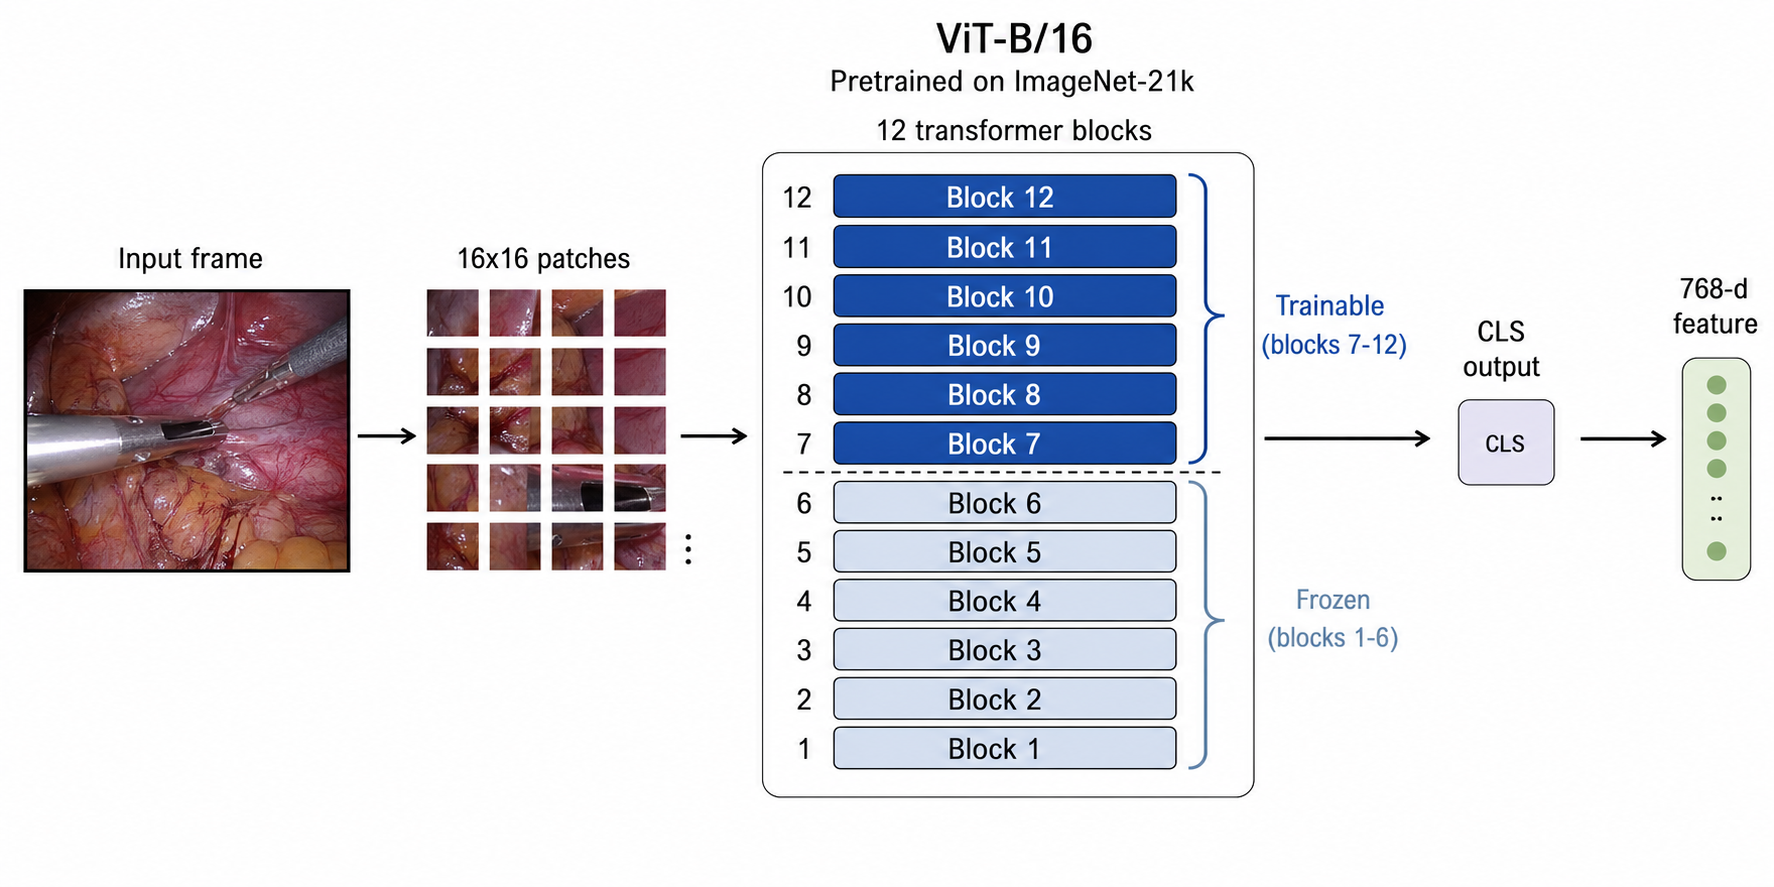
\includegraphics[width=0.9\linewidth]{vit_freeze_diagram.png}
\caption{ViT-B/16 frame encoder initialized from ImageNet-21k. The
lower 6 transformer blocks are frozen and the upper 6 are fine-tuned;
the final [CLS] output is used as the 768-dimensional frame feature.}
\label{fig:app-vit-freeze}
\end{figure}

\begin{figure}[p]
\centering
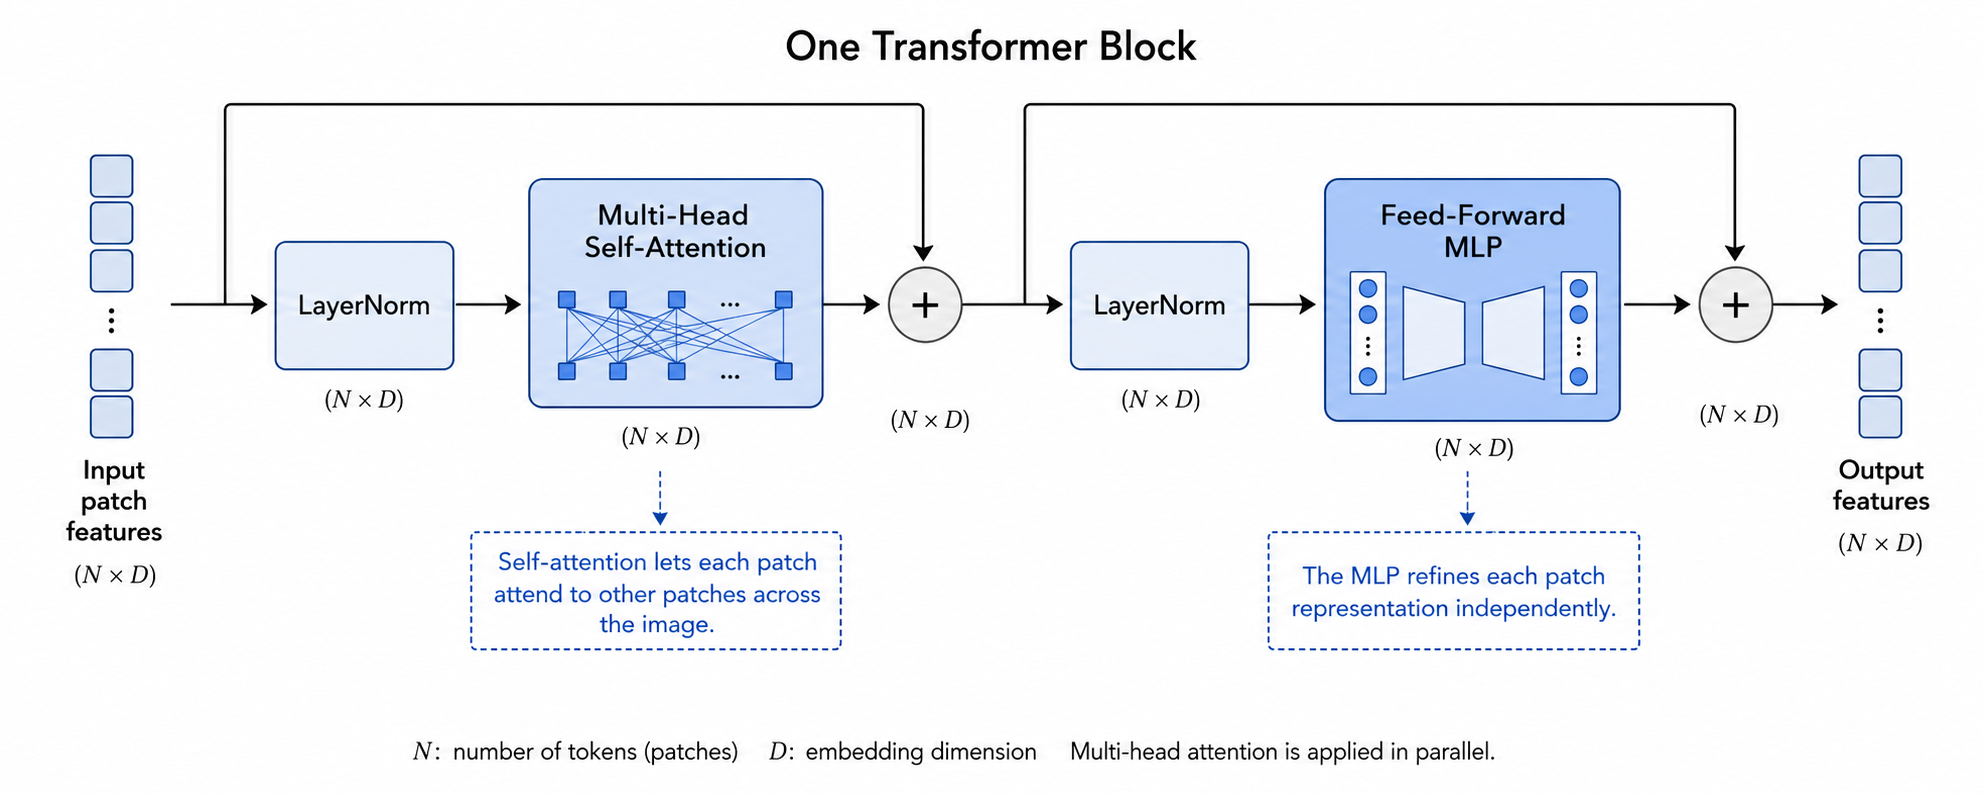
\includegraphics[width=0.8\linewidth]{transformer_block_diagram.png}
\caption{One transformer block in the ViT encoder. Self-attention lets
each image patch interact with other patches across the frame, and the
feed-forward MLP refines the representation.}
\label{fig:app-transformer-block}
\end{figure}

\begin{figure}[p]
\centering
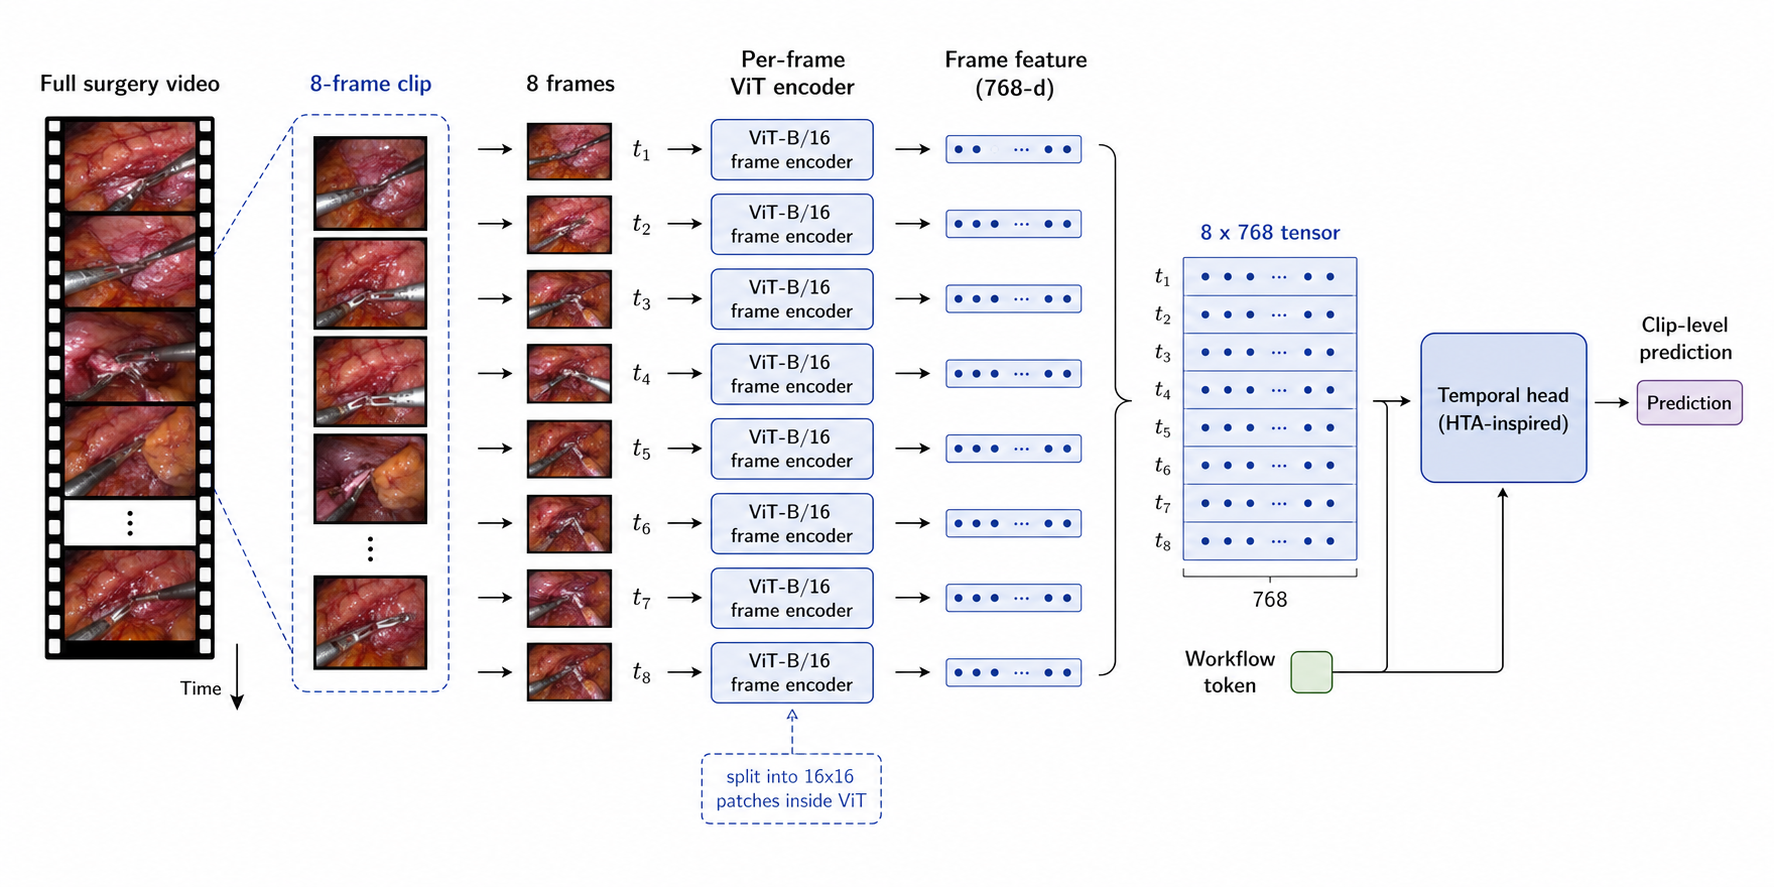
\includegraphics[width=\linewidth]{clip_to_tensor_pipeline.png}
\caption{From a full surgery video, we sample an 8-frame clip. Each
frame is encoded independently by ViT-B/16, producing one
768-dimensional feature per frame. Stacking these features yields an
\(8 \times 768\) tensor, which is then combined with the workflow token
and passed to the temporal head for clip-level prediction.}
\label{fig:app-clip-pipeline}
\end{figure}

\begin{figure}[p]
\centering
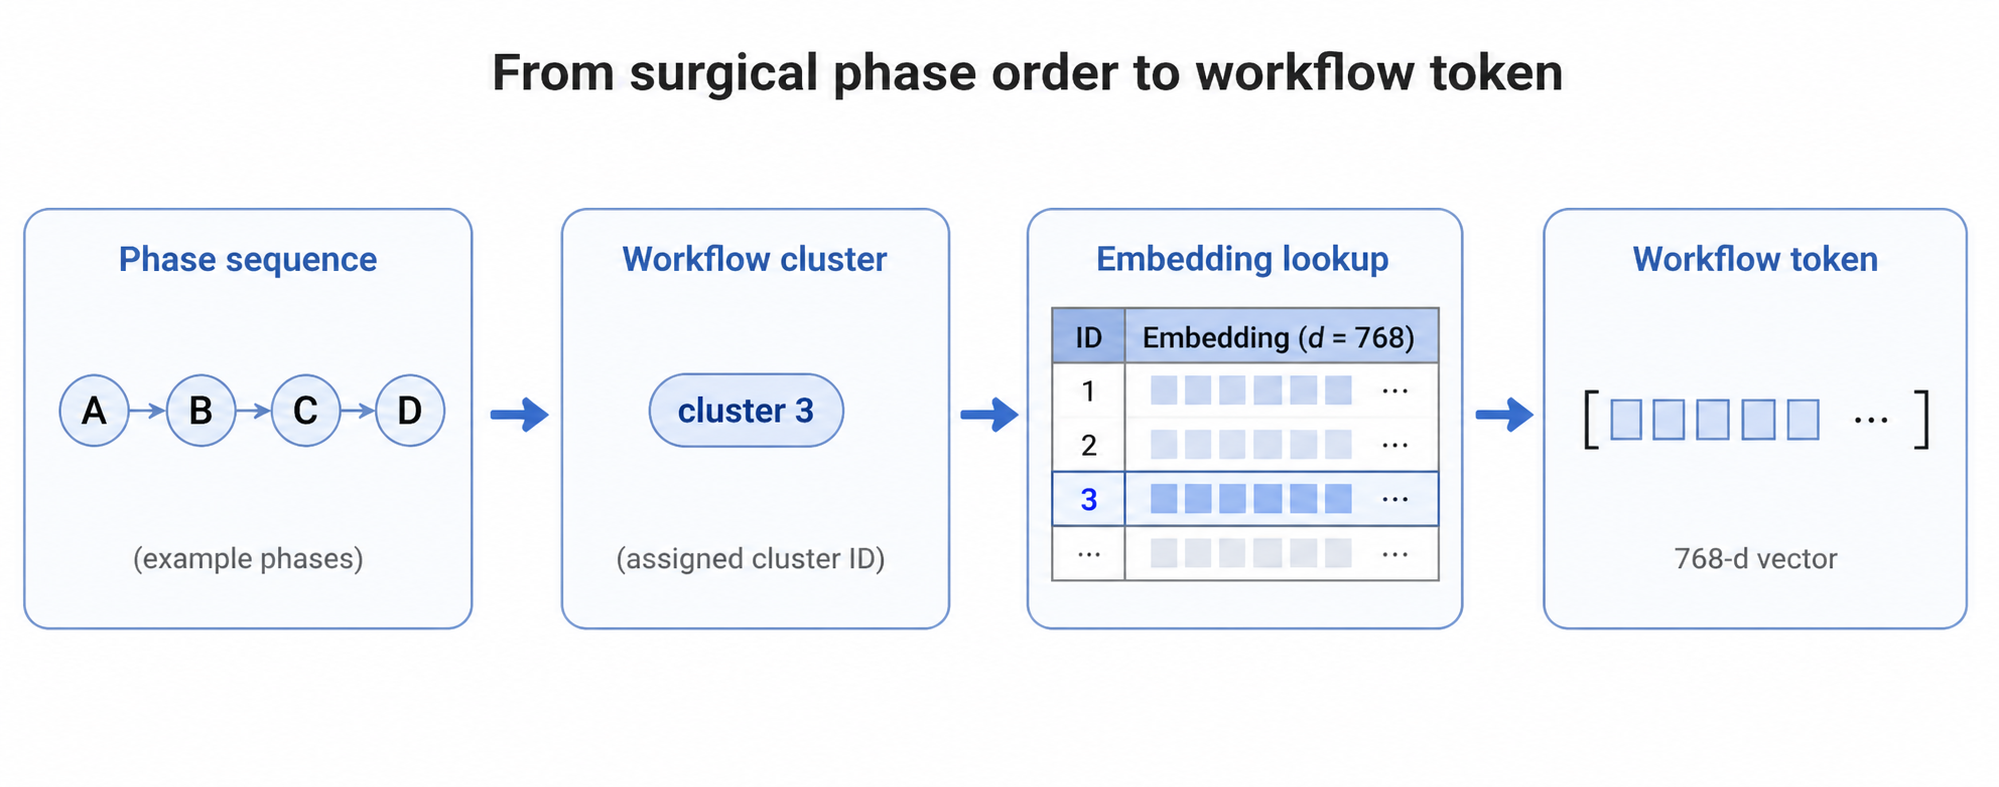
\includegraphics[width=0.7\linewidth]{workflow_token_diagram.png}
\caption{Workflow-token construction. The phase sequence is mapped to a
workflow cluster, which is then converted into a learned embedding
vector used as the workflow token.}
\label{fig:app-workflow-token}
\end{figure}

\begin{figure}[p]
\centering
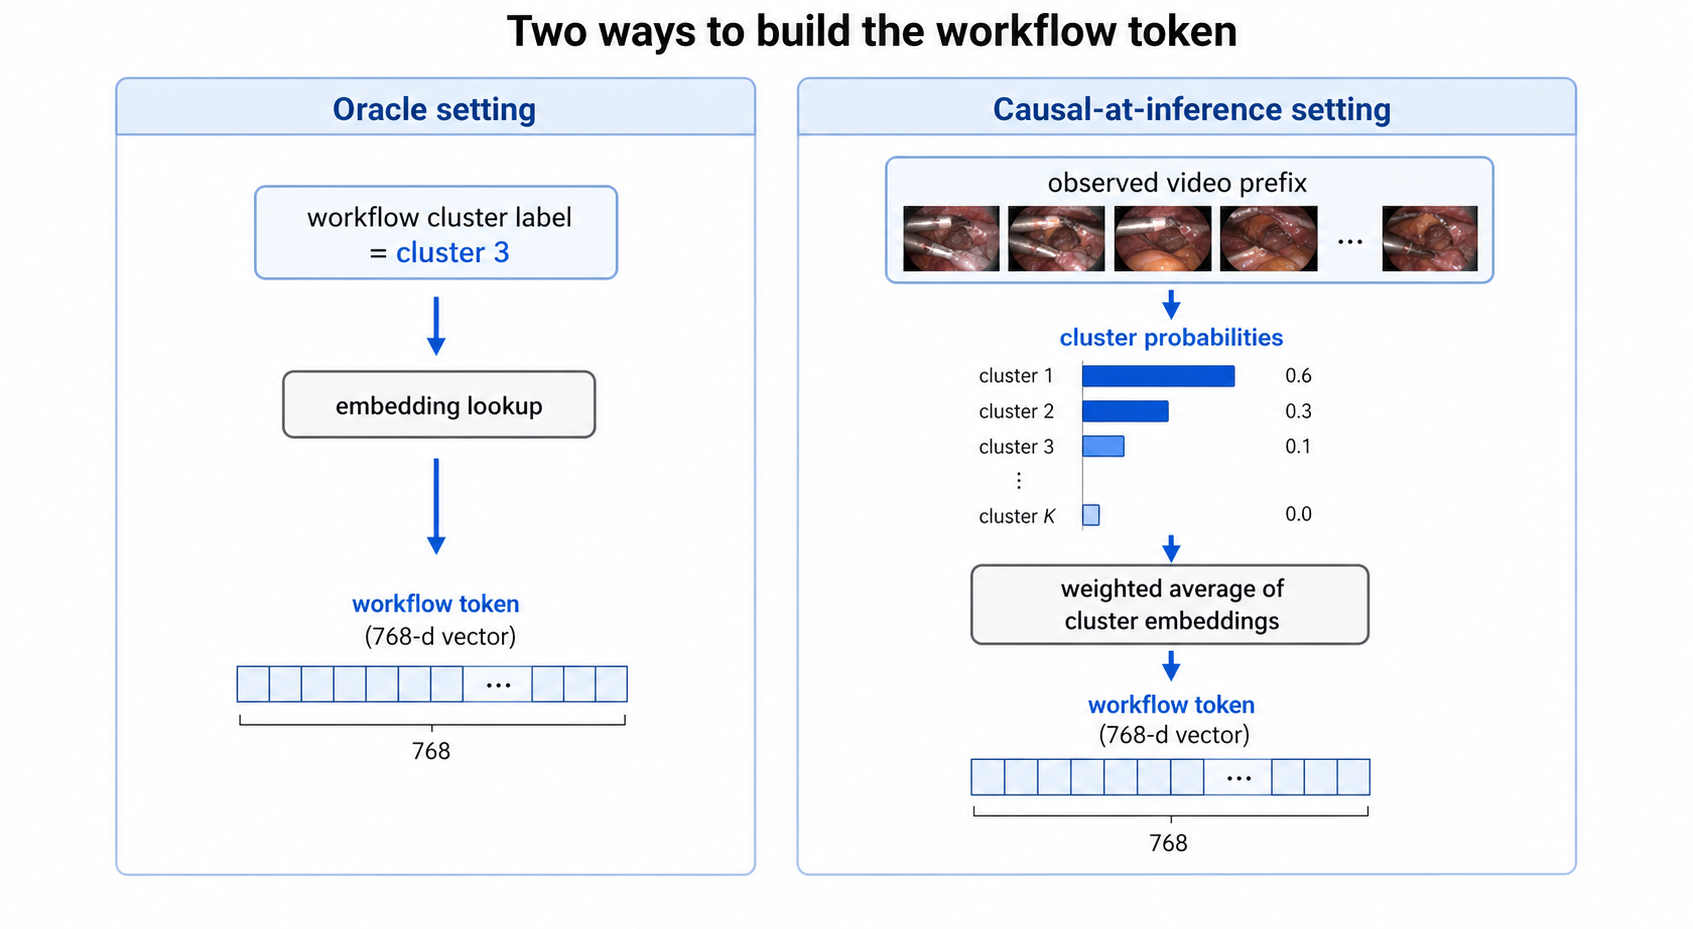
\includegraphics[width=0.85\linewidth]{workflow_token_oracle_vs_causal.png}
\caption{Oracle versus causal-at-inference workflow tokens. In the
oracle setting, the model receives the embedding for a single known
cluster. In the causal-at-inference setting, it uses a probability
distribution over clusters derived from the observed surgical prefix and
forms a weighted average of cluster embeddings.}
\label{fig:app-workflow-token-oracle-causal}
\end{figure}

\begin{figure}[p]
\centering
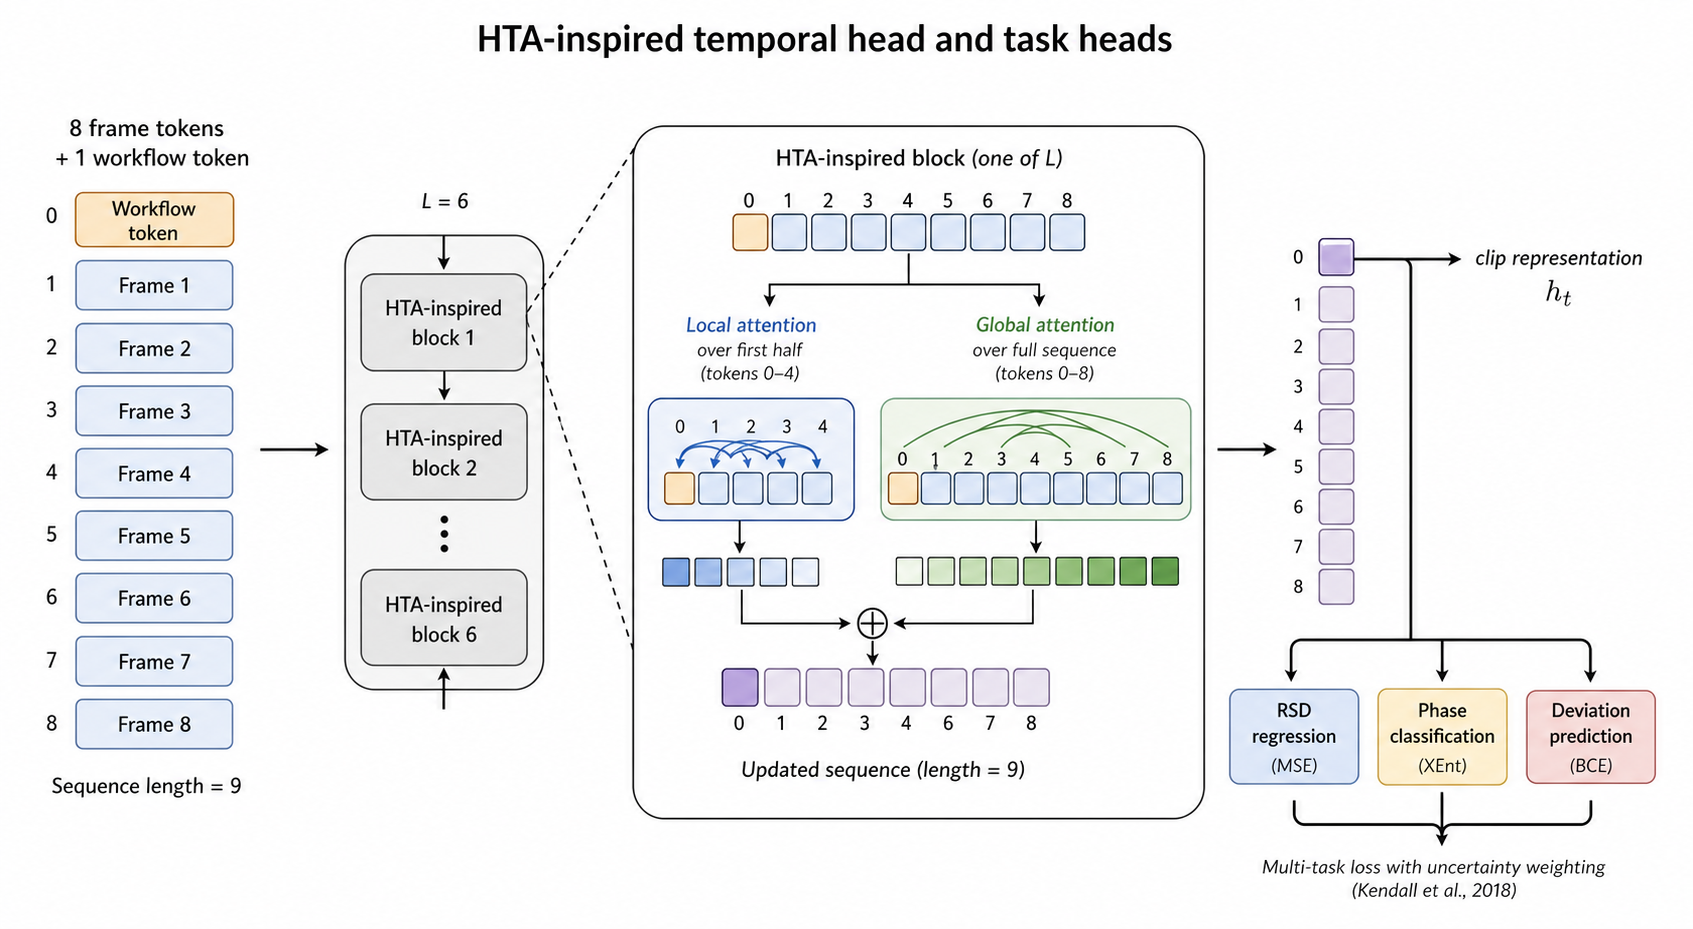
\includegraphics[width=\linewidth]{hta_temporal_head_diagram.png}
\caption{HTA-inspired temporal head. The input sequence contains 8
frame-level features and 1 workflow token. Each temporal block combines
a local-attention branch over part of the sequence with a
global-attention branch over the full sequence. The output at position 0
is used as the clip-level representation \(\mathbf{h}_t\), which feeds
the RSD, phase, and deviation heads.}
\label{fig:app-hta-head}
\end{figure}

\clearpage

\bibliographystyle{plainnat}
\bibliography{references}

\end{document}
